% Options for packages loaded elsewhere
\PassOptionsToPackage{unicode}{hyperref}
\PassOptionsToPackage{hyphens}{url}
\PassOptionsToPackage{dvipsnames,svgnames,x11names}{xcolor}
%
\documentclass[
  letterpaper,
  DIV=11,
  numbers=noendperiod]{scrartcl}

\usepackage{amsmath,amssymb}
\usepackage{iftex}
\ifPDFTeX
  \usepackage[T1]{fontenc}
  \usepackage[utf8]{inputenc}
  \usepackage{textcomp} % provide euro and other symbols
\else % if luatex or xetex
  \usepackage{unicode-math}
  \defaultfontfeatures{Scale=MatchLowercase}
  \defaultfontfeatures[\rmfamily]{Ligatures=TeX,Scale=1}
\fi
\usepackage{lmodern}
\ifPDFTeX\else  
    % xetex/luatex font selection
\fi
% Use upquote if available, for straight quotes in verbatim environments
\IfFileExists{upquote.sty}{\usepackage{upquote}}{}
\IfFileExists{microtype.sty}{% use microtype if available
  \usepackage[]{microtype}
  \UseMicrotypeSet[protrusion]{basicmath} % disable protrusion for tt fonts
}{}
\makeatletter
\@ifundefined{KOMAClassName}{% if non-KOMA class
  \IfFileExists{parskip.sty}{%
    \usepackage{parskip}
  }{% else
    \setlength{\parindent}{0pt}
    \setlength{\parskip}{6pt plus 2pt minus 1pt}}
}{% if KOMA class
  \KOMAoptions{parskip=half}}
\makeatother
\usepackage{xcolor}
\setlength{\emergencystretch}{3em} % prevent overfull lines
\setcounter{secnumdepth}{5}
% Make \paragraph and \subparagraph free-standing
\ifx\paragraph\undefined\else
  \let\oldparagraph\paragraph
  \renewcommand{\paragraph}[1]{\oldparagraph{#1}\mbox{}}
\fi
\ifx\subparagraph\undefined\else
  \let\oldsubparagraph\subparagraph
  \renewcommand{\subparagraph}[1]{\oldsubparagraph{#1}\mbox{}}
\fi

\usepackage{color}
\usepackage{fancyvrb}
\newcommand{\VerbBar}{|}
\newcommand{\VERB}{\Verb[commandchars=\\\{\}]}
\DefineVerbatimEnvironment{Highlighting}{Verbatim}{commandchars=\\\{\}}
% Add ',fontsize=\small' for more characters per line
\usepackage{framed}
\definecolor{shadecolor}{RGB}{241,243,245}
\newenvironment{Shaded}{\begin{snugshade}}{\end{snugshade}}
\newcommand{\AlertTok}[1]{\textcolor[rgb]{0.68,0.00,0.00}{#1}}
\newcommand{\AnnotationTok}[1]{\textcolor[rgb]{0.37,0.37,0.37}{#1}}
\newcommand{\AttributeTok}[1]{\textcolor[rgb]{0.40,0.45,0.13}{#1}}
\newcommand{\BaseNTok}[1]{\textcolor[rgb]{0.68,0.00,0.00}{#1}}
\newcommand{\BuiltInTok}[1]{\textcolor[rgb]{0.00,0.23,0.31}{#1}}
\newcommand{\CharTok}[1]{\textcolor[rgb]{0.13,0.47,0.30}{#1}}
\newcommand{\CommentTok}[1]{\textcolor[rgb]{0.37,0.37,0.37}{#1}}
\newcommand{\CommentVarTok}[1]{\textcolor[rgb]{0.37,0.37,0.37}{\textit{#1}}}
\newcommand{\ConstantTok}[1]{\textcolor[rgb]{0.56,0.35,0.01}{#1}}
\newcommand{\ControlFlowTok}[1]{\textcolor[rgb]{0.00,0.23,0.31}{#1}}
\newcommand{\DataTypeTok}[1]{\textcolor[rgb]{0.68,0.00,0.00}{#1}}
\newcommand{\DecValTok}[1]{\textcolor[rgb]{0.68,0.00,0.00}{#1}}
\newcommand{\DocumentationTok}[1]{\textcolor[rgb]{0.37,0.37,0.37}{\textit{#1}}}
\newcommand{\ErrorTok}[1]{\textcolor[rgb]{0.68,0.00,0.00}{#1}}
\newcommand{\ExtensionTok}[1]{\textcolor[rgb]{0.00,0.23,0.31}{#1}}
\newcommand{\FloatTok}[1]{\textcolor[rgb]{0.68,0.00,0.00}{#1}}
\newcommand{\FunctionTok}[1]{\textcolor[rgb]{0.28,0.35,0.67}{#1}}
\newcommand{\ImportTok}[1]{\textcolor[rgb]{0.00,0.46,0.62}{#1}}
\newcommand{\InformationTok}[1]{\textcolor[rgb]{0.37,0.37,0.37}{#1}}
\newcommand{\KeywordTok}[1]{\textcolor[rgb]{0.00,0.23,0.31}{#1}}
\newcommand{\NormalTok}[1]{\textcolor[rgb]{0.00,0.23,0.31}{#1}}
\newcommand{\OperatorTok}[1]{\textcolor[rgb]{0.37,0.37,0.37}{#1}}
\newcommand{\OtherTok}[1]{\textcolor[rgb]{0.00,0.23,0.31}{#1}}
\newcommand{\PreprocessorTok}[1]{\textcolor[rgb]{0.68,0.00,0.00}{#1}}
\newcommand{\RegionMarkerTok}[1]{\textcolor[rgb]{0.00,0.23,0.31}{#1}}
\newcommand{\SpecialCharTok}[1]{\textcolor[rgb]{0.37,0.37,0.37}{#1}}
\newcommand{\SpecialStringTok}[1]{\textcolor[rgb]{0.13,0.47,0.30}{#1}}
\newcommand{\StringTok}[1]{\textcolor[rgb]{0.13,0.47,0.30}{#1}}
\newcommand{\VariableTok}[1]{\textcolor[rgb]{0.07,0.07,0.07}{#1}}
\newcommand{\VerbatimStringTok}[1]{\textcolor[rgb]{0.13,0.47,0.30}{#1}}
\newcommand{\WarningTok}[1]{\textcolor[rgb]{0.37,0.37,0.37}{\textit{#1}}}

\providecommand{\tightlist}{%
  \setlength{\itemsep}{0pt}\setlength{\parskip}{0pt}}\usepackage{longtable,booktabs,array}
\usepackage{calc} % for calculating minipage widths
% Correct order of tables after \paragraph or \subparagraph
\usepackage{etoolbox}
\makeatletter
\patchcmd\longtable{\par}{\if@noskipsec\mbox{}\fi\par}{}{}
\makeatother
% Allow footnotes in longtable head/foot
\IfFileExists{footnotehyper.sty}{\usepackage{footnotehyper}}{\usepackage{footnote}}
\makesavenoteenv{longtable}
\usepackage{graphicx}
\makeatletter
\def\maxwidth{\ifdim\Gin@nat@width>\linewidth\linewidth\else\Gin@nat@width\fi}
\def\maxheight{\ifdim\Gin@nat@height>\textheight\textheight\else\Gin@nat@height\fi}
\makeatother
% Scale images if necessary, so that they will not overflow the page
% margins by default, and it is still possible to overwrite the defaults
% using explicit options in \includegraphics[width, height, ...]{}
\setkeys{Gin}{width=\maxwidth,height=\maxheight,keepaspectratio}
% Set default figure placement to htbp
\makeatletter
\def\fps@figure{htbp}
\makeatother
% definitions for citeproc citations
\NewDocumentCommand\citeproctext{}{}
\NewDocumentCommand\citeproc{mm}{%
  \begingroup\def\citeproctext{#2}\cite{#1}\endgroup}
\makeatletter
 % allow citations to break across lines
 \let\@cite@ofmt\@firstofone
 % avoid brackets around text for \cite:
 \def\@biblabel#1{}
 \def\@cite#1#2{{#1\if@tempswa , #2\fi}}
\makeatother
\newlength{\cslhangindent}
\setlength{\cslhangindent}{1.5em}
\newlength{\csllabelwidth}
\setlength{\csllabelwidth}{3em}
\newenvironment{CSLReferences}[2] % #1 hanging-indent, #2 entry-spacing
 {\begin{list}{}{%
  \setlength{\itemindent}{0pt}
  \setlength{\leftmargin}{0pt}
  \setlength{\parsep}{0pt}
  % turn on hanging indent if param 1 is 1
  \ifodd #1
   \setlength{\leftmargin}{\cslhangindent}
   \setlength{\itemindent}{-1\cslhangindent}
  \fi
  % set entry spacing
  \setlength{\itemsep}{#2\baselineskip}}}
 {\end{list}}
\usepackage{calc}
\newcommand{\CSLBlock}[1]{\hfill\break\parbox[t]{\linewidth}{\strut\ignorespaces#1\strut}}
\newcommand{\CSLLeftMargin}[1]{\parbox[t]{\csllabelwidth}{\strut#1\strut}}
\newcommand{\CSLRightInline}[1]{\parbox[t]{\linewidth - \csllabelwidth}{\strut#1\strut}}
\newcommand{\CSLIndent}[1]{\hspace{\cslhangindent}#1}

\KOMAoption{captions}{tableheading}
\makeatletter
\@ifpackageloaded{caption}{}{\usepackage{caption}}
\AtBeginDocument{%
\ifdefined\contentsname
  \renewcommand*\contentsname{Table of contents}
\else
  \newcommand\contentsname{Table of contents}
\fi
\ifdefined\listfigurename
  \renewcommand*\listfigurename{List of Figures}
\else
  \newcommand\listfigurename{List of Figures}
\fi
\ifdefined\listtablename
  \renewcommand*\listtablename{List of Tables}
\else
  \newcommand\listtablename{List of Tables}
\fi
\ifdefined\figurename
  \renewcommand*\figurename{Figure}
\else
  \newcommand\figurename{Figure}
\fi
\ifdefined\tablename
  \renewcommand*\tablename{Table}
\else
  \newcommand\tablename{Table}
\fi
}
\@ifpackageloaded{float}{}{\usepackage{float}}
\floatstyle{ruled}
\@ifundefined{c@chapter}{\newfloat{codelisting}{h}{lop}}{\newfloat{codelisting}{h}{lop}[chapter]}
\floatname{codelisting}{Listing}
\newcommand*\listoflistings{\listof{codelisting}{List of Listings}}
\makeatother
\makeatletter
\makeatother
\makeatletter
\@ifpackageloaded{caption}{}{\usepackage{caption}}
\@ifpackageloaded{subcaption}{}{\usepackage{subcaption}}
\makeatother
\ifLuaTeX
  \usepackage{selnolig}  % disable illegal ligatures
\fi
\usepackage{bookmark}

\IfFileExists{xurl.sty}{\usepackage{xurl}}{} % add URL line breaks if available
\urlstyle{same} % disable monospaced font for URLs
\hypersetup{
  pdftitle={Multi-model ensembles in infectious disease and public health: methods, interpretation, and implementation in R},
  pdfauthor={Li Shandross; Emily Howerton; Lucie Contamin; Harry Hochheiser; Anna Krystalli; Consortium of Infectious Disease Modeling Hubs; Nicholas G. Reich; Evan L. Ray},
  pdfkeywords={multiple models, aggregation, forecast, prediction},
  colorlinks=true,
  linkcolor={blue},
  filecolor={Maroon},
  citecolor={Blue},
  urlcolor={Blue},
  pdfcreator={LaTeX via pandoc}}

\title{Multi-model ensembles in infectious disease and public health:
methods, interpretation, and implementation in R}
\author{Li Shandross \and Emily Howerton \and Lucie Contamin \and Harry
Hochheiser \and Anna Krystalli \and Consortium of Infectious Disease
Modeling Hubs \and Nicholas G. Reich \and Evan L. Ray}
\date{}

\begin{document}
\maketitle
\begin{abstract}
Combining predictions from multiple models into an ensemble is a widely
used practice across many fields with demonstrated performance benefits.
Popularized through domains such as weather forecasting and climate
modeling, multi-model ensembles are becoming increasingly common in
public health and biological applications. For example, multi-model
outbreak forecasting provides more accurate and reliable information
about the timing and burden of infectious disease outbreaks to public
health officials and medical practitioners. Yet, understanding and
interpreting multi-model ensemble results can be difficult, as there are
a diversity of methods proposed in the literature with no clear
consensus on which is best. Moreover, a lack of standard, easy-to-use
software implementations impedes the generation of multi-model ensembles
in practice. To address these challenges, we provide an introduction to
the statistical foundations of applied probabilistic forecasting,
including the role of multi-model ensembles. We introduce the
\texttt{hubEnsembles} package, a flexible framework for ensembling
various types of predictions using a range of methods. Finally, we
present a tutorial and case-study of ensemble methods using the
\texttt{hubEnsembles} package on a subset of real, publicly available
data from the FluSight Forecast Hub.
\end{abstract}

\section{Introduction}\label{sec-intro}

Predictions of future outcomes are essential to planning and decision
making, yet generating reliable predictions of the future is
challenging. One method for overcoming this challenge is combining
predictions across multiple, independent models. These combination
methods (also called aggregation or ensembling) have been repeatedly
shown to produce predictions that are more accurate\textsuperscript{1,2}
and more consistent\textsuperscript{3} than individual models. Because
of the clear performance benefits, multi-model ensembles are a widely
used statistical tool across fields, including weather
forecasting\textsuperscript{4}, climate modeling\textsuperscript{5}, and
economics\textsuperscript{6}. In the last decade, the number of
multi-model ensemble predictions generated and used in real time for
public health planning and response has grown rapidly.

In particular, predicting infectious disease outbreaks and anticipating
the effects of potential interventions has demonstrated utility for
public health officials and medical practitioners. Underlying these
predictions are mathematical models that use historical disease
incidence data to make probabilistic predictions of incidence in the
future\textsuperscript{7--11}. Given the performance benefits of
multi-model ensembles, it is becoming increasingly common to convene
multiple modeling teams into a collaborative
``hub''\textsuperscript{12}, where each team generates independent
predictions that are aggregated to collectively produce an ensemble. For
example, this approach has been used to make real-time, multi-model
predictions for seasonal influenza\textsuperscript{10,13},
dengue\textsuperscript{14}, West Nile virus\textsuperscript{15}, and
more recently SARS-CoV-2\textsuperscript{16--18}.

Generating multi-model ensembles or interpreting the resulting
predictions depends on understanding the underlying statistical
methodology. There are many proposed methods for generating ensembles,
and these methods differ in at least one of two ways: (1) the function
used to combine or ``average'' predictions, and (2) how predictions are
weighted when performing the combination. A few methodological papers
have discussed theory of multi-model ensembles and tested various
ensembling methods in public health applications
specifically\textsuperscript{19--25}, yet there is no consensus on which
method should be favored. There are software packages that support
various aspects of multi-model ensembling\textsuperscript{26--29}.
However, these packages only support a subset of methods and prediction
types, illustrating the need for standard, easy-to-use implementations
of common methods.

Here, we provide an introduction to the statistical foundations of
multi-model ensembles in applied probabilistic forecasting
(Section~\ref{sec-defs}). In addition, to improve accessibility,
reproducibility, and interoperability, we have developed a comprehensive
R package \texttt{hubEnsembles} that implements these methods. The
\texttt{hubEnsembles} package provides a flexible framework for
generating ensemble predictions from multiple models across a range of
common methods and prediction types; it is situated within the broader
``hubverse'' collection of open-source software and data tools to
facilitate the development and management of collaborative modeling
exercises\textsuperscript{30}. These two factors together, a simple
implementation framework across methods and integration with hubverse
data standards and tools, make \texttt{hubEnsembles} accessible and easy
to use. Finally, we present a basic demonstration of multi-model
ensemble generation and interpretation (Section~\ref{sec-simple-ex}),
and a more in-depth analysis using real influenza forecasts
(Section~\ref{sec-case-study}). Together, these case studies motivate a
discussion and comparison of the various methods
(Section~\ref{sec-conclusions}). While the case studies focus on
infectious disease applications, the software and tools presented are
general and could be used for applications in other areas of biomedical
and public health research, or other domains. By reviewing multi-model
ensemble methodology and synthesizing these methods into an easy-to use
implementation, this tutorial provides guidance on understanding,
interpreting, and implementing multi-model ensembles.

\section{How to generate a multi-model ensemble}\label{sec-defs}

In this section, we provide an overview of the process to generate a
multi-model ensemble, including basic definitions of key statistical
concepts in probabilistic forecasting, and an overview of the classes of
methods that are typically used for generating a multi-model ensemble.

\subsection{Key statistical concepts in
forecasting}\label{key-statistical-concepts-in-forecasting}

Generating an ensemble requires multiple predictions to be combined, and
a combination method for calculating the ensemble from these predictions
(Figure~\ref{fig-ensemble-schematic}). These predictions will often be
produced by different statistical or mathematical models, and the output
from these models (referred to as ``model output'' from here on) will
vary based on the setting. For example, some public health questions,
such as short-term resource allocation, may depend on a forecast of
public health outcomes weeks into the future, whereas longer-term
decisions about vaccination schedules may require projections months
into the future across multiple possible scenarios. Some intervention
decisions, such as quarantine and isolation policy, may depend on
estimates of key biological parameters such as the generation interval
for an infectious pathogen. Throughout, we will use the general term
``prediction'' to encapsulate all such outcomes that could be modeled.
Predictions can also capture varying degrees of uncertainty in the
outcome. A \emph{point prediction} gives a single estimate of an outcome
while a \emph{probabilistic prediction} provides an estimated
probability distribution over a set of outcomes. In either case, the
basic steps required to generate an ensemble are the same.

\begin{figure}

\centering{

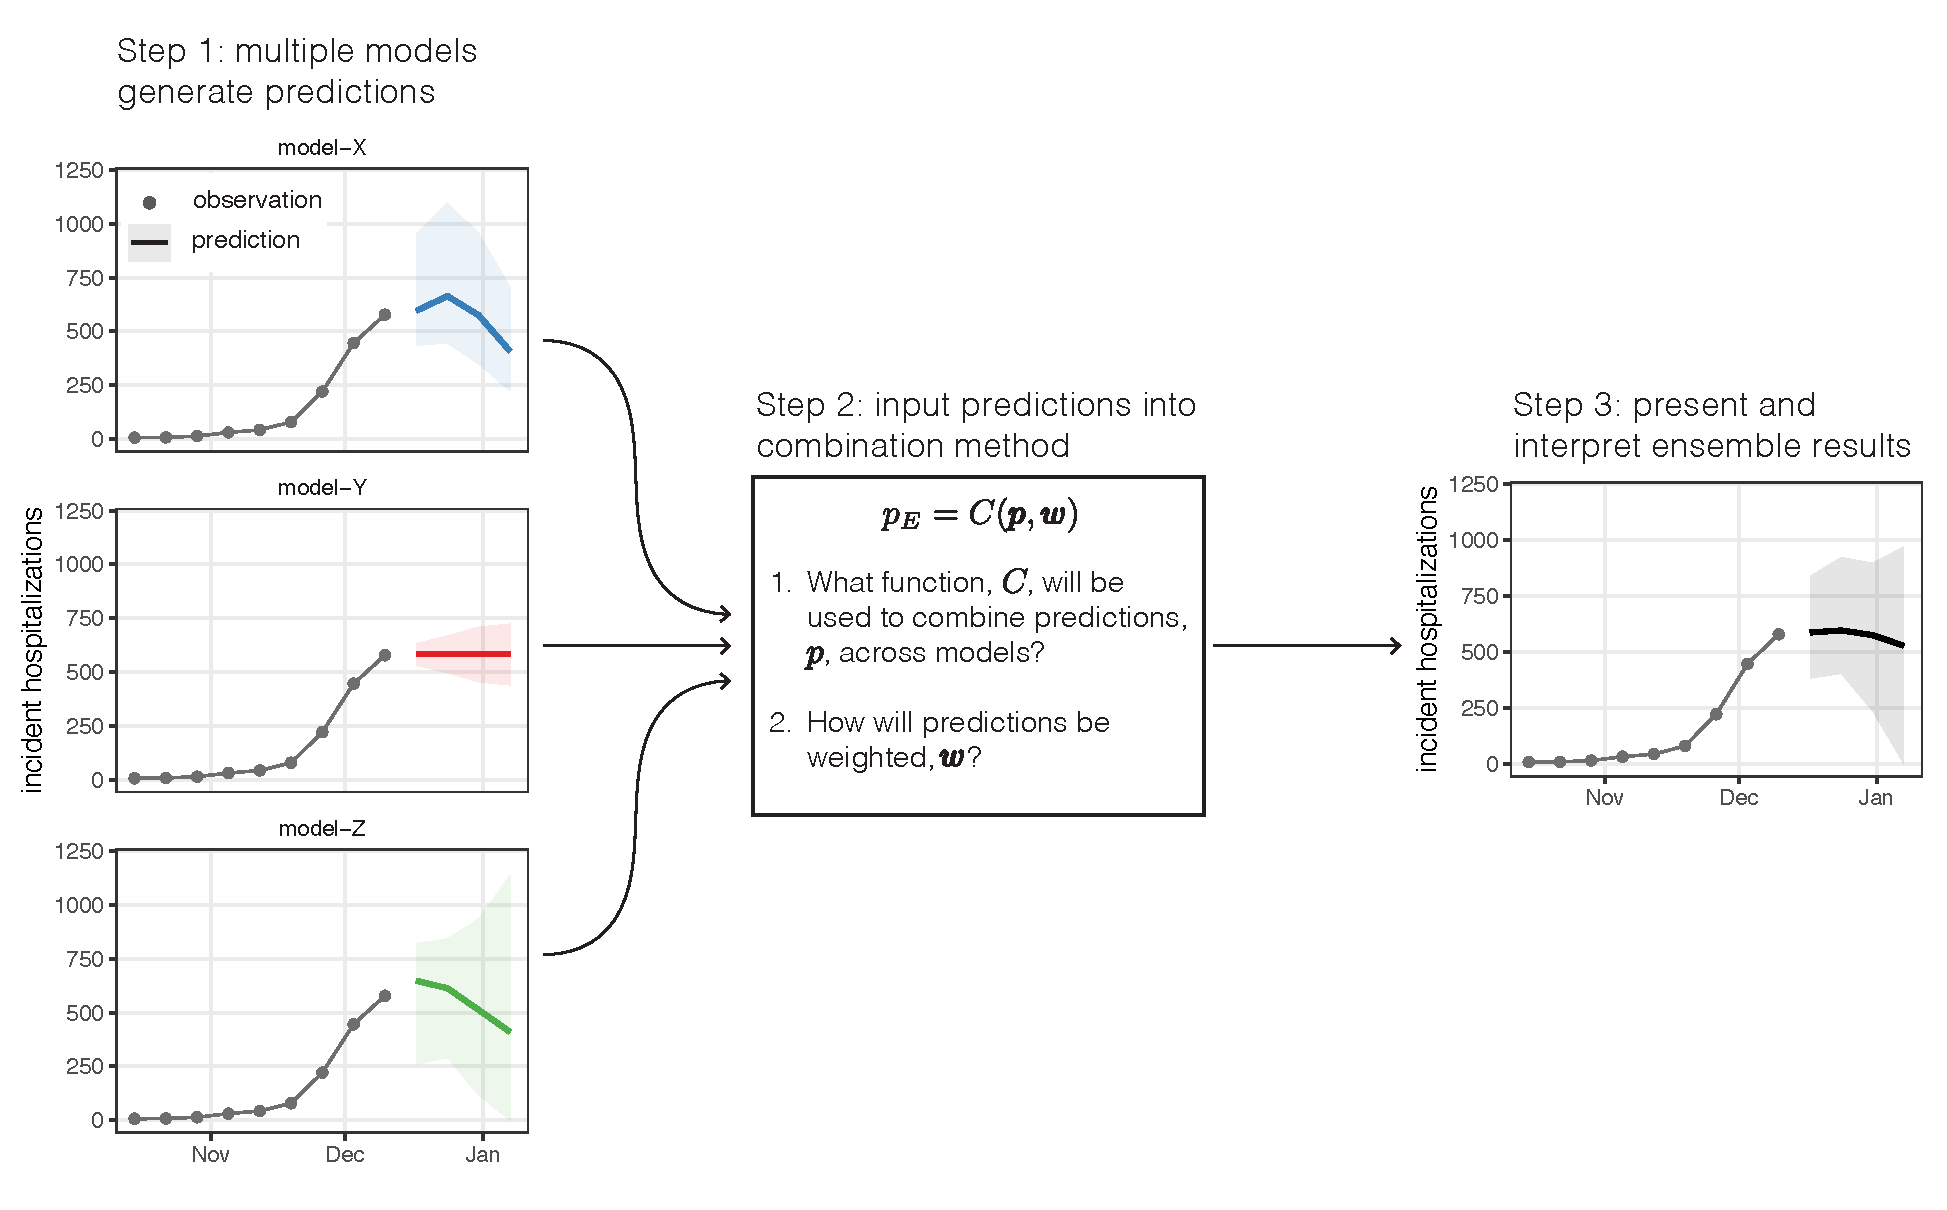
\includegraphics{overview_fig_FULL.pdf}

}

\caption{\label{fig-ensemble-schematic}Overview of process to generate a
multi-model ensemble. Predictions, \(p_i\) are generated from \(N\)
independent models (step 1). Then those predictions,
\(\pmb{p} = \{p_i|i \in 1, ..., N\}\), are combined with some function,
\(C\), and set of weights, \(\pmb{w} = \{w_i|i \in 1, ..., N\}\). This
figure illustrates example probabilistic forecasts for incident
influenza hospitalizations, where the median (line) and 90\% prediction
interval are shown. In this case, the ensemble is constructed using the
linear pool method (\(F_{LOP}(x)\)\}).}

\end{figure}%

\subsection{Mathematical definitions and properties of ensemble
methods}\label{mathematical-definitions-and-properties-of-ensemble-methods}

Here, we use \(N\) to denote the total number of individual predictions
that the ensemble will combine. For example, if predictions are produced
by different models, \(N\) is the total number of models that have
provided predictions. Individual predictions will be indexed by the
subscript \(i\). Optionally, one can calculate an ensemble that uses a
weight \(w_i\) for each prediction; we define the set of model-specific
weights as \(\pmb{w} = \{w_i | i \in 1, ..., N\}\). Informally,
predictions with a larger weight have a greater influence on the
ensemble prediction, though the details of this depend on the ensemble
method (described further below).

Then, for a set of \(N\) point predictions,
\(\pmb{p} = \{p_i|i \in 1, ..., N\}\), each from a distinct model \(i\),
an ensemble of these predictions is

\[
p_E = C(\pmb{p}, \pmb{w}) 
\]

using any function \(C\) and any set of model-specific weights
\(\pmb{w}\). For example, an arithmetic average of predictions yields
\(p_E = \sum_{i=1}^Np_iw_i\), where the weights are non-negative and sum
to 1. If \(w_i = 1/N\) for all \(i\), all predictions will be equally
weighted. More complex functions for aggregation are also possible, such
as a (weighted) median or geometric mean.

For probabilistic predictions, there are two commonly used classes of
methods to average or ensemble multiple predictions: quantile averaging
(also called a Vincent average\textsuperscript{31}) and probability
averaging (also called a distributional mixture or linear opinion
pool\textsuperscript{32})\textsuperscript{33}. To define these two
classes of methods, let \(F(x)\) be a cumulative density function (CDF)
defined over values \(x\) of the target variable for the prediction, and
\(F^{-1}(\theta)\) be the corresponding quantile function defined over
quantile levels \(\theta \in [0, 1]\). Throughout this article, we may
refer to \(x\) as either a `value of the target variable' or a
`quantile' depending on the context, and similarly we may refer to
\(\theta\) as either a `quantile level' or a `(cumulative) probability'.
Additionally, we will use \(f(x)\) to denote a probability mass function
(PMF) for a prediction of a discrete variable or a discretization (such
as binned values) of a continuous variable.

The quantile average combines a set of quantile functions,
\(\mathcal{Q} = \{F_i^{-1}(\theta)| i \in 1,...,N \}\), with a given set
of weights, \(\pmb{w}\), as \[
F^{-1}_Q(\theta) = C_Q(\mathcal{Q}, \pmb{w}) = \sum_{i = 1}^Nw_iF^{-1}_i(\theta).
\]

This computes the average value of predictions across different models
for each fixed quantile level \(\theta\). For a normal distribution or
any distribution with a location and scale parameter, the resulting
quantile average will be the same type of distribution, with location
and scale parameters that are the average of the location and scale
parameters from the individual distributions
(Figure~\ref{fig-example-quantile-average-and-linear-pool}, panel B). In
other words, this method interprets the predictive probability
distributions that are being combined as uncertain estimates of a single
true distribution. It is also possible to use other combination
functions, such as a weighted median, to combine quantile predictions.

The probability average or linear pool is calculated by averaging
probabilities across predictions for a fixed value of the target
variable, \(x\). In other words, for a set of CDFs
\(\mathcal{F} = \{F_i(x)| i \in 1,...,N \}\) and weights \(\pmb{w}\),
the linear pool is calculated as

\[
F_{LOP}(x) = C_{LOP}(\mathcal{F}, \pmb{w}) = \sum_{i = 1}^Nw_iF_i(x). 
\]

For a set of PMF values, \(\{f_i(x)|i \in 1, ..., N\}\), the linear pool
can be equivalently calculated as
\(f_{LOP}(x) = \sum_{i = 1}^N w_i f_i(x)\). Statistically this amounts
to a mixture of the probability distributions, and the resulting
probability distribution can be interpreted as one where the constituent
probability distributions represent alternative predictions of the
future, each of which has a probability \(w_i\) of being the true one.
For a visual depiction of these equations, see
Figure~\ref{fig-example-quantile-average-and-linear-pool} below.

\begin{figure}

\centering{

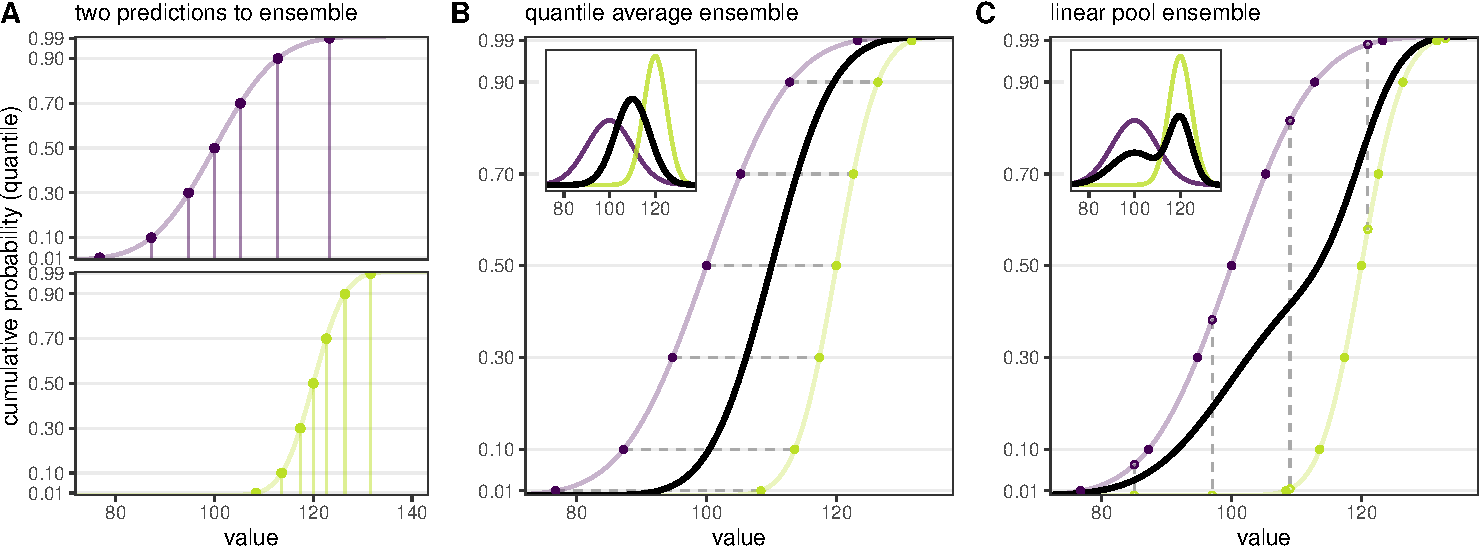
\includegraphics{hubEnsembles_manuscript_files/figure-pdf/fig-example-quantile-average-and-linear-pool-1.pdf}

}

\caption{\label{fig-example-quantile-average-and-linear-pool}(Panel A)
Example predictions from two distributions (\(N(100, 10)\) in purple and
\(N(120, 5)\) in green) shown as cumulative distribution functions
(CDFs). To ease submission to a hub, the prediction can be summarized at
a fixed number of points along the distribution. Here, the solid points
show model output for seven fixed quantile levels (\(\theta\) = 0.01,
0.1, 0.3, 0.5, 0.7, 0.9, and 0.99). The y-axis ticks show each of the
fixed quantile levels. The associated values for each fixed quantile
level are shown with vertical lines. (Panel B) Quantile average
ensemble, which is calculated by averaging values for each fixed
quantile level (represented by horizontal dashed gray lines). The
distributions and corresponding model outputs from panel A are
re-plotted and the black line shows the resulting quantile average
ensemble. Inset shows corresponding probability density functions
(PDFs). (Panel C) Linear pool ensemble, which is calculated by averaging
cumulative probabilities for each fixed value (represented by vertical
dashed gray lines). The distributions and corresponding model outputs
from panel A are re-plotted. To calculate the linear pool in this case,
where model outputs are not defined for the same values (i.e., vertical
lines in Panel A do not line up), the model outputs are used to
interpolate the full CDF for each distribution from which predicted
cumulative probabilities can be extracted for fixed values (shown with
open circles). The black line shows the resulting linear pool average
ensemble. Inset shows corresponding PDFs.}

\end{figure}%

The different averaging methods for probabilistic predictions yield
different properties of the resulting ensemble distribution. For
example, the variance of the linear pool is
\(\sigma^2_{LOP} = \sum_{i=1}^Nw_i\sigma_i^2 + \sum_{i=1}^Nw_i(\mu_i-\mu_{LOP})^2\),
where \(\mu_i\) is the mean and \(\sigma^2_i\) is the variance of
individual prediction \(i\), and although there is no closed-form
variance for the quantile average, the variance of the quantile average
will always be less than or equal to that of the linear
pool\textsuperscript{33}. Both methods generate distributions with the
same mean, \(\mu_Q = \mu_{LOP} = \sum_{i=1}^Nw_i\mu_i\), which is the
mean of individual model means\textsuperscript{33}. The linear pool
method preserves variation between individual models, whereas the
quantile average cancels away this variation under the assumption it
constitutes sampling error\textsuperscript{24}.

\subsection{Applications in public health and infectious disease
outbreaks}\label{applications-in-public-health-and-infectious-disease-outbreaks}

Multi-model ensembles have become the gold standard for forecasting and
prediction efforts that support public health in real
time\textsuperscript{12,34--36}. One prominent domain is forecasting key
characteristics of infectious disease outbreaks, including weekly
incidence or healthcare demand over future weeks, disease burden for the
entire season, and timing and magnitude of the outbreak
peak\textsuperscript{14--16,23,37}. Projections of disease outcomes
under multiple possible future scenarios have also been used to estimate
intervention effectiveness to inform policy\textsuperscript{38--40}, and
it has been proposed to use short-term forecasts of incidence to inform
vaccine efficacy trials\textsuperscript{41}. Standard guidelines for
reporting of prediction efforts in outbreak and public health settings
have also been established\textsuperscript{42}.

Across a variety of pathogens and outbreak settings, multi-model
ensembles have been shown to produce forecasts that are as good or
better than the individual models that compose the
ensemble\textsuperscript{10,13,14,16--19,23}. Notably, the ensemble does
not always outperform the best model, but typically offers improved
consistency and robustness over individual
models\textsuperscript{16,17,20,43}. However, in one instance, a
baseline historical average of West Nile Virus cases in the US
outperformed most model predictions, including the
ensemble\textsuperscript{15}.

Examinations of ensemble methodology in infectious disease contexts
suggest there is not one method that universally performs best. In
short-term forecasting settings, a simple linear pool average of
component predictions tends to produce prediction intervals that are too
wide (i.e., suggesting outcomes are more uncertain than in reality);
beta-transformation\textsuperscript{44} and dynamic
weighting\textsuperscript{45} have been suggested to mitigate this
problem. A median quantile average has been shown to provide similar
performance to a weighted mean in short-term forecasting challenges,
while also offering robustness to changes in performance across
individuals models\textsuperscript{25}, and was thus used as the primary
ensemble for short-term forecasts of COVID-19\textsuperscript{16,17}.
For longer-term predictions of COVID-19, a trimmed LOP ensemble
performed best, as models tended to be more overconfident in this
setting\textsuperscript{18}. The number of models submitting real-time
predictions has varied dramatically (from as few as four models for
longer-term predictions of COVID-19\textsuperscript{18} to more than 40
for short-term forecasts of COVID-19\textsuperscript{16}). Research
including applications across influenza and COVID-19 suggests that at
least 3 models are needed, with diminishing returns for every model that
is added\textsuperscript{46}.

The growing body of literature on multi-model ensembles in public health
domains emphasizes the utility of these approaches to inform response in
real time. Future research on optimizing ensemble performance for
different targets and time horizons will further improve utility.
Moreover, expanding the use of these methods to other pathogens and
countries will enable further methodological development.

\section{How to implement ensemble
calculations}\label{sec-implementation}

The methods described in Section~\ref{sec-defs} are implemented via the
\texttt{hubEnsembles} package in a flexible, easy-to-use framework.
Importantly, \texttt{hubEnsembles} is situated within the broader
hubverse software infrastructure, which provides data standards and
conventions for representing and working with model
predictions\textsuperscript{30}, including for example, collecting and
manipulating predictions (\texttt{hubUtils}) as well as visualization
(\texttt{hubVis}). In 2024-2025, the hubverse supported over a dozen
collaborative modeling hubs used by public health agencies across the
globe. We begin with a short overview of hubverse concepts and
conventions that support the process of combining model predictions,
supplemented by example predictions provided by the hubverse in
\texttt{hubExamples}, then explain the implementation of the two primary
ensembling functions included in the package,
\texttt{simple\_ensemble()} and \texttt{linear\_pool()}.

\subsection{Terminology and data standards in the
hubverse}\label{terminology-and-data-standards-in-the-hubverse}

In the hubverse, predictions are always represented in a standardized
tabular format called ``model output'', codified by the
\texttt{model\_out\_tbl} S3 class in \texttt{hubUtils} (a package of
basic utility functions). Each row represents a single, unique
prediction while the columns provide information about what is being
predicted, its scope, and value. A single model output object can store
and organize many predictions while remaining easy to parse at a glance,
which is particularly useful when collecting predictions from multiple
models to combine into an ensemble. Any tabular predictions can be
transformed into model output using the \texttt{as\_model\_out\_tbl()}
function from \texttt{hubUtils} (see Section~\ref{sec-case-study} for an
example).

The \texttt{model\_out\_tbl} class is defined by four standard types of
columns: (i) the model ID, which denotes which model has produced the
prediction; (ii) the task IDs (also referred to as ``task ID variables''
or ``task ID columns''), which provide details about what is being
predicted; (iii) the model output representation, which specify the type
of prediction and other identifying information; and (iv) the value of
the prediction itself. While most of these columns are always required
and have standardized column names, the task ID variables may vary
according to the needs of the modeling hub or modeling
task\textsuperscript{30}.

Table~\ref{tbl-example-forecasts} provides an example of model output
that stores short-term forecasts of weekly flu hospitalizations for
different US states and territories. By reading across the table, we can
see that these are quantile predictions (\texttt{output\_type}) of the
quartiles (output type ID: \texttt{otid}) from a single model
(\texttt{model\_id} of ``team1-mod'') for four distinct forecast
horizons. Here, details about the prediction related to modeling task
are represented by the task ID variables \texttt{loc} (location
abbreviation), \texttt{ref\_date} (reference date: the ``starting
point'' of the forecasts), \texttt{h} (horizon: how many weeks into the
future, relative to the \texttt{ref\_date}), and \texttt{target} (what
is being predicted).

\begin{longtable}[]{@{}
  >{\raggedright\arraybackslash}p{(\columnwidth - 14\tabcolsep) * \real{0.1507}}
  >{\raggedright\arraybackslash}p{(\columnwidth - 14\tabcolsep) * \real{0.0822}}
  >{\raggedright\arraybackslash}p{(\columnwidth - 14\tabcolsep) * \real{0.1507}}
  >{\raggedleft\arraybackslash}p{(\columnwidth - 14\tabcolsep) * \real{0.0548}}
  >{\raggedright\arraybackslash}p{(\columnwidth - 14\tabcolsep) * \real{0.1644}}
  >{\raggedright\arraybackslash}p{(\columnwidth - 14\tabcolsep) * \real{0.1918}}
  >{\raggedright\arraybackslash}p{(\columnwidth - 14\tabcolsep) * \real{0.0959}}
  >{\raggedleft\arraybackslash}p{(\columnwidth - 14\tabcolsep) * \real{0.1096}}@{}}

\caption{\label{tbl-example-forecasts}Example of forecasts for incident
influenza hospitalizations, formatted according to hubverse standards.
Quantile predictions for the median and 50\% prediction intervals from a
single model are shown for four distinct horizons. The
\texttt{output\_type\_id} column's name has been shortened to
\texttt{otid} for brevity. These predictions are a modified subset of
the \texttt{forecast\_outputs} data provided by the \texttt{hubExamples}
package.}

\tabularnewline

\toprule\noalign{}
\begin{minipage}[b]{\linewidth}\raggedright
\texttt{model\_id}
\end{minipage} & \begin{minipage}[b]{\linewidth}\raggedright
\texttt{loc}
\end{minipage} & \begin{minipage}[b]{\linewidth}\raggedright
\texttt{ref\_date}
\end{minipage} & \begin{minipage}[b]{\linewidth}\raggedleft
\texttt{h}
\end{minipage} & \begin{minipage}[b]{\linewidth}\raggedright
\texttt{target}
\end{minipage} & \begin{minipage}[b]{\linewidth}\raggedright
\texttt{output\_type}
\end{minipage} & \begin{minipage}[b]{\linewidth}\raggedright
\texttt{otid}
\end{minipage} & \begin{minipage}[b]{\linewidth}\raggedleft
\texttt{value}
\end{minipage} \\
\midrule\noalign{}
\endhead
\bottomrule\noalign{}
\endlastfoot
team1-mod & MA & 2022-12-17 & 0 & wk flu hosp & quantile & 0.25 & 514 \\
team1-mod & MA & 2022-12-17 & 0 & wk flu hosp & quantile & 0.5 & 596 \\
team1-mod & MA & 2022-12-17 & 0 & wk flu hosp & quantile & 0.75 & 713 \\
team1-mod & MA & 2022-12-17 & 1 & wk flu hosp & quantile & 0.25 & 563 \\
team1-mod & MA & 2022-12-17 & 1 & wk flu hosp & quantile & 0.5 & 664 \\
team1-mod & MA & 2022-12-17 & 1 & wk flu hosp & quantile & 0.75 & 803 \\
team1-mod & MA & 2022-12-17 & 2 & wk flu hosp & quantile & 0.25 & 469 \\
team1-mod & MA & 2022-12-17 & 2 & wk flu hosp & quantile & 0.5 & 575 \\
team1-mod & MA & 2022-12-17 & 2 & wk flu hosp & quantile & 0.75 & 705 \\
team1-mod & MA & 2022-12-17 & 3 & wk flu hosp & quantile & 0.25 & 324 \\
team1-mod & MA & 2022-12-17 & 3 & wk flu hosp & quantile & 0.5 & 408 \\
team1-mod & MA & 2022-12-17 & 3 & wk flu hosp & quantile & 0.75 & 512 \\

\end{longtable}

As mentioned previously, task ID variables are not fixed in name,
number, or composition to incorporate flexibility in the
\texttt{model\_out\_tbl} class. Different modeling efforts may use
different sets of task ID columns with different values to define their
prediction goals, or may simply choose distinct names to represent the
same concept. For example, the date task column was named
\texttt{ref\_date} above but could easily be called
\texttt{origin\_date} or \texttt{forecast\_date} instead. Some standard
examples of task ID variables are available on the hubverse
documentation website\textsuperscript{30}.

The ``model output representation'' columns \texttt{output\_type} and
\texttt{output\_type\_id} contain metadata about how the predictions are
conveyed. The hubverse data standards require that these columns are
included in a \texttt{model\_out\_tbl}. The \texttt{output\_type} column
defines how a prediction is represented and may be \texttt{"mean"} or
\texttt{"median"} for point predictions, or one of \texttt{"quantile"},
\texttt{"cdf"}, \texttt{"pmf"}, or \texttt{"sample"} for probabilistic
predictions. The \texttt{output\_type\_id} provides additional
identifying information for prediction and is specific to the particular
\texttt{output\_type} (see Table~\ref{tbl-model-output-rep}). The last
column, \texttt{value}, always contains the numeric value of the
prediction, regardless of output type. Requirements for the values of
the \texttt{output\_type\_id} and \texttt{value} columns associated with
each valid output type are summarized in
Table~\ref{tbl-model-output-rep}.

\begin{longtable}[]{@{}
  >{\raggedright\arraybackslash}p{(\columnwidth - 4\tabcolsep) * \real{0.2603}}
  >{\raggedright\arraybackslash}p{(\columnwidth - 4\tabcolsep) * \real{0.3288}}
  >{\raggedright\arraybackslash}p{(\columnwidth - 4\tabcolsep) * \real{0.4110}}@{}}
\caption{A table summarizing how the model output representation columns
are used for predictions of different output types; adapted from
hubverse documentation\textsuperscript{30}. (*Rows of sample predictions
from a particular model that share an output type ID value may be
assumed to represent a single sample from a joint distribution across
multiple levels of the task ID variables.)
}\label{tbl-model-output-rep}\tabularnewline
\toprule\noalign{}
\begin{minipage}[b]{\linewidth}\raggedright
\texttt{output\_type}
\end{minipage} & \begin{minipage}[b]{\linewidth}\raggedright
\texttt{output\_type\_id}
\end{minipage} & \begin{minipage}[b]{\linewidth}\raggedright
\texttt{value}
\end{minipage} \\
\midrule\noalign{}
\endfirsthead
\toprule\noalign{}
\begin{minipage}[b]{\linewidth}\raggedright
\texttt{output\_type}
\end{minipage} & \begin{minipage}[b]{\linewidth}\raggedright
\texttt{output\_type\_id}
\end{minipage} & \begin{minipage}[b]{\linewidth}\raggedright
\texttt{value}
\end{minipage} \\
\midrule\noalign{}
\endhead
\bottomrule\noalign{}
\endlastfoot
\texttt{mean} & NA (not used for mean predictions) & Numeric: The mean
of the predictive distribution \\
\texttt{median} & NA (not used for median predictions) & Numeric: The
median of the predictive distribution \\
\texttt{quantile} & Numeric between 0.0 and 1.0: A quantile level &
Numeric: The quantile of the predictive distribution at the quantile
level specified by the \texttt{output\_type\_id} \\
\texttt{cdf} & String or numeric naming a possible value of the target
variable & Numeric between 0.0 and 1.0: The cumulative probability of
the predictive distribution at the value of the outcome variable
specified by the \texttt{output\_type\_id} \\
\texttt{pmf} & String naming a possible category of a discrete outcome
variable & Numeric between 0.0 and 1.0: The probability mass of the
predictive distribution when evaluated at a specified level of a
categorical outcome variable \\
\texttt{sample} & Integer or string identifying the sample* & Numeric: A
single sample value from the predictive distribution \\
\end{longtable}

All output types can summarize predictions from univariate marginal
distributions, e.g.~for a single location and time point. The sample
output type, which represents randomly drawn values from a probabilistic
predictive distribution, is unique in that it can additionally represent
predictions from joint predictive distributions. This means that samples
may encode dependence across combinations of multiple values for task ID
variables, for example across multiple locations and/or time points. In
this case, rows of sample predictions with the same index (specified by
the \texttt{output\_type\_id}) from a particular model may be assumed to
correspond to a single sample from a joint distribution.

For quantile predictions, the \texttt{output\_type\_id} is a numeric
value between 0 and 1 specifying the cumulative probability associated
with the quantile prediction. In the notation we defined in
Section~\ref{sec-defs}, the \texttt{output\_type\_id} corresponds to
\(\theta\) and the \texttt{value} is the quantile prediction
\(F^{-1}(\theta)\). For CDF or PMF predictions, the
\texttt{output\_type\_id} is the target variable value \(x\) at which
the cumulative distribution function or probability mass function for
the predictive distribution should be evaluated, and the \texttt{value}
column contains the predicted \(F(x)\) or \(f(x)\), respectively.

The hubverse also provides standards for target data, which can be
stored in one of two formats: target time series or oracle output. The
two tabular representations differ in terms of columns and purposes.
Target time series data is a more traditional representation of the
observed ``truth'' in a time series format with minimal columns; this
format usually serves as calibration data for generating forecasts.
Oracle output, on the other hand, represents prediction that an ``oracle
model'' would have made had it known the observed values in advance.
This format resembles model output data and is suited for evaluating
forecasts. Some examples of target data are given in
Section~\ref{sec-simple-ex}.

\subsection{Ensemble functions in hubEnsembles}\label{sec-ens-fns}

The \texttt{hubEnsembles} package contains two functions that perform
ensemble calculations: \texttt{simple\_ensemble()}, which applies some
function to each model prediction, and \texttt{linear\_pool()}, which
computes an ensemble using the linear opinion pool method. In the
following sections, we outline the implementation details for each
function and how these implementations correspond to the statistical
ensembling methods described in Section~\ref{sec-defs}. A short
description of the calculation performed by each function is summarized
by output type in Table~\ref{tbl-fns-by-output-type}.

\begin{longtable}[]{@{}
  >{\raggedright\arraybackslash}p{(\columnwidth - 4\tabcolsep) * \real{0.1400}}
  >{\raggedright\arraybackslash}p{(\columnwidth - 4\tabcolsep) * \real{0.5000}}
  >{\raggedright\arraybackslash}p{(\columnwidth - 4\tabcolsep) * \real{0.3600}}@{}}
\caption{Summary of ensemble function calculations for each output type.
The ensemble function determines the operation that is performed, and in
the case of probabilistic output types (quantile, CDF, PMF), this also
determines what ensemble distribution is generated (quantile average,
\(F_{Q}^{-1}(\theta)\), or linear pool, \(F_{LOP}(x)\)). The ensembled
predictions are returned in the same output type as the inputs. Thus,
the output type determines how the resulting ensemble distribution is
summarized (as a quantile, \(F^{-1}(\theta)\), cumulative probability,
\(F(x)\), or probability \(f(x)\)). Estimating individual model
cumulative probabilities is required to compute a
\texttt{linear\_pool()} for predictions of \texttt{quantile} output
type; see Section~\ref{sec-linear-pool} on the linear pool operation for
details. In the case of \texttt{simple\_ensemble()}, we show the
calculations for the default case where \texttt{agg\_fun\ =\ mean};
however, if another aggregation function is chosen (e.g.,
\texttt{agg\_fun\ =\ median}), that calculation would be performed
instead. For example,
\texttt{simple\_ensemble(...,\ agg\_fun\ =\ median)} applied to
predictions of mean output type would return the median of individual
model means.}\label{tbl-fns-by-output-type}\tabularnewline
\toprule\noalign{}
\begin{minipage}[b]{\linewidth}\raggedright
\texttt{output\_type}
\end{minipage} & \begin{minipage}[b]{\linewidth}\raggedright
\texttt{simple\_ensemble(...,\ agg\_fun=mean)}
\end{minipage} & \begin{minipage}[b]{\linewidth}\raggedright
\texttt{linear\_pool()}
\end{minipage} \\
\midrule\noalign{}
\endfirsthead
\toprule\noalign{}
\begin{minipage}[b]{\linewidth}\raggedright
\texttt{output\_type}
\end{minipage} & \begin{minipage}[b]{\linewidth}\raggedright
\texttt{simple\_ensemble(...,\ agg\_fun=mean)}
\end{minipage} & \begin{minipage}[b]{\linewidth}\raggedright
\texttt{linear\_pool()}
\end{minipage} \\
\midrule\noalign{}
\endhead
\bottomrule\noalign{}
\endlastfoot
\texttt{mean} & mean of individual model means & mean of individual
model means \\
\texttt{median} & mean of individual model medians & NA \\
\texttt{quantile} & mean of individual model target variable values at
each quantile level, \(F^{-1}_Q(\theta)\) & quantiles of the
distribution are obtained by computing the mean of estimated individual
model cumulative probabilities at each target variable value,
\(F^{-1}_{LOP}(\theta)\) \\
\texttt{cdf} & mean of individual model cumulative probabilities at each
target variable value, \(F_{LOP}(x)\) & mean of individual model
cumulative probabilities at each target variable value,
\(F_{LOP}(x)\) \\
\texttt{pmf} & mean of individual model bin or category probabilities at
each target variable value, \(f_{LOP}(x)\) & mean of individual model
bin or category probabilities at each target variable value,
\(f_{LOP}(x)\) \\
\texttt{sample} & NA & samples of the distribution are obtained by
stratified draw from individual models' samples \\
\end{longtable}

\subsubsection{Simple ensemble}\label{sec-simple-ensemble}

The \texttt{simple\_ensemble()} function directly computes an ensemble
from component model outputs by combining them via some function (\(C\))
within each unique combination of task ID variables, output types, and
output type IDs. This function can be used to summarize predictions of
output types mean, median, quantile, CDF, and PMF. The mechanics of the
ensemble calculations are the same for each of the output types, though
the resulting statistical ensembling method differs for different output
types (Table~\ref{tbl-fns-by-output-type}).

By default, \texttt{simple\_ensemble()} uses the mean for the
aggregation function \(C\) and equal weights for all models. For point
predictions with a mean or median output type, the resulting ensemble
prediction is an equally weighted average of the individual models'
predictions. For probabilistic predictions in a quantile format, by
default \texttt{simple\_ensemble()} calculates an equally weighted
average of individual model target variable values at each quantile
level, which is equivalent to a quantile average. For model outputs in a
CDF or PMF format, by default \texttt{simple\_ensemble()} computes an
equally weighted average of individual model (cumulative or bin)
probabilities at each target variable value, which is equivalent to the
linear pool method.

Any aggregation function \(C\) may be specified by the user. For
example, a median ensemble may also be created by specifying
\texttt{median} as the aggregation function, or a custom function may be
passed to the \texttt{agg\_fun} argument to create other ensemble types.
Similarly, model weights can be specified to create a weighted ensemble.

\subsubsection{Linear pool}\label{sec-linear-pool}

The \texttt{linear\_pool()} function implements the linear opinion pool
(LOP) method for ensembling predictions. Currently, this function can be
used to combine predictions with output types mean, quantile, CDF, PMF,
and sample. Unlike \texttt{simple\_ensemble()}, this function handles
its computation differently based on the output type. For the CDF, PMF,
and mean output types, the linear pool method is equivalent to calling
\texttt{simple\_ensemble()} with a mean aggregation function (see
Table~\ref{tbl-fns-by-output-type}), since \texttt{simple\_ensemble()}
produces a linear pool prediction (an average of individual model
cumulative or bin probabilities).

For the sample output type, the LOP method collects a stratified draw of
the individual models' predictions and pools them into a single ensemble
distribution. By default, all samples are used to create this ensemble.
Additionally, only equally-weighted linear pools of samples are
supported by the \texttt{hubEnsembles} package during this time. Samples
may also be converted to another common output type such as quantiles or
bin probabilities (as the main scientific interest often concerns a
summary of samples), and other ensemble methods may then be utilized for
that output type.

For the quantile output type, implementation of LOP is comparatively
less straightforward. This is because LOP averages cumulative
probabilities at each value of the target variable, but the predictions
are given as quantiles (on the scale of the target variable) for fixed
quantile levels. The value for these quantile predictions will generally
differ between models; hence, we are typically not provided cumulative
probabilities at the same values of the target variable for all
component predictions. This lack of alignment between cumulative
probabilities for the same target variable values impedes computation of
LOP from quantile predictions and is illustrated in panel A of
Figure~\ref{fig-example-quantile-average-and-linear-pool}.

Given that LOP cannot be directly calculated from quantile predictions,
we must first obtain an estimate of the CDF for each component
distribution from the provided quantiles, combine the CDFs, then
calculate the quantiles using the ensemble's CDF. We perform this
calculation in three main steps, assisted by the \texttt{distfromq}
package\textsuperscript{47} for the first two:

\begin{enumerate}
\def\labelenumi{\arabic{enumi}.}
\tightlist
\item
  Interpolate and extrapolate from the provided quantiles for each
  component model to obtain an estimate of the CDF of that particular
  distribution.
\item
  Draw samples from each component model distribution. To reduce Monte
  Carlo variability, we use quasi-random samples corresponding to
  quantiles of the estimated distribution\textsuperscript{48}.
\item
  Pool the samples from all component models and extract the desired
  quantiles.
\end{enumerate}

For step 1, functionality in the \texttt{distfromq} package uses a
monotonic cubic spline for interpolation on the interior of the provided
quantiles. The user may choose one of several distributions to perform
extrapolation of the CDF tails. These include normal, lognormal, and
Cauchy distributions, with ``normal'' set as the default. A
location-scale parameterization is used, with separate location and
scale parameters chosen in the lower and upper tails so as to match the
two most extreme quantiles. The sampling process described in steps 2
and 3 approximates the linear pool calculation described in
Section~\ref{sec-defs}.

\section{A simple demonstration of multi-model
ensembles}\label{sec-simple-ex}

In this section, we provide a simple example to illustrate how to
compute a multi-model ensemble and compare the methods supported by the
functions of \texttt{hubEnsembles}.

\subsection{Example data: a forecast
hub}\label{example-data-a-forecast-hub}

The first step in generating a multi-model ensemble is to gather the
predictions we wish to combine. In this example, we use some short-term
forecasts already formatted as model output data from the
\texttt{hubExamples} package. These model outputs are from a larger
example modeling hub, created using a modified subset of predictions
from the FluSight Forecasting challenge (discussed in further detail in
Section~\ref{sec-case-study}). In addition to toy model output data, the
example hub also includes observed data in the form of target time
series data and oracle output.

The model output is stored in a data object named
\texttt{forecast\_outputs} and contains mean, median, quantile, and
sample forecasts of future incident influenza hospitalizations, as well
as CDF and PMF forecasts of hospitalization intensity. Each prediction
is described by five task ID variables: the location for which the
forecast was made (\texttt{location}), the date on which the forecast
was made (\texttt{reference\_date}), the number of steps ahead
(\texttt{horizon}), the date of the forecast prediction
(\texttt{target\_end\_date}, a combination of the date the forecast was
made and the forecast horizon), and the forecast target
(\texttt{target}). We begin by examining the predictions for weekly
incident influenza hospitalizations, displaying a subset of each output
type in Table~\ref{tbl-example-model-outputs}.

\begin{longtable}[]{@{}
  >{\raggedright\arraybackslash}p{(\columnwidth - 10\tabcolsep) * \real{0.2169}}
  >{\raggedright\arraybackslash}p{(\columnwidth - 10\tabcolsep) * \real{0.1928}}
  >{\raggedleft\arraybackslash}p{(\columnwidth - 10\tabcolsep) * \real{0.1205}}
  >{\raggedright\arraybackslash}p{(\columnwidth - 10\tabcolsep) * \real{0.1687}}
  >{\raggedright\arraybackslash}p{(\columnwidth - 10\tabcolsep) * \real{0.2048}}
  >{\raggedleft\arraybackslash}p{(\columnwidth - 10\tabcolsep) * \real{0.0964}}@{}}

\caption{\label{tbl-example-model-outputs}Example model output for
forecasts of weekly incident influenza hospitalizations. A subset of
example model output is shown: 1-week ahead forecasts made on 2022-12-17
for Massachusetts from three distinct models; only the mean, median,
select samples, and the 5th, 25th, 75th and 95th quantiles are
displayed. The \texttt{location}, \texttt{reference\_date} and
\texttt{target\_end\_date} columns have been omitted for brevity. This
example data is provided in the \texttt{hubExamples} package.}

\tabularnewline

\toprule\noalign{}
\begin{minipage}[b]{\linewidth}\raggedright
\texttt{model\_id}
\end{minipage} & \begin{minipage}[b]{\linewidth}\raggedright
\texttt{target}
\end{minipage} & \begin{minipage}[b]{\linewidth}\raggedleft
\texttt{horizon}
\end{minipage} & \begin{minipage}[b]{\linewidth}\raggedright
\texttt{output\_type}
\end{minipage} & \begin{minipage}[b]{\linewidth}\raggedright
\texttt{output\_type\_id}
\end{minipage} & \begin{minipage}[b]{\linewidth}\raggedleft
\texttt{value}
\end{minipage} \\
\midrule\noalign{}
\endhead
\bottomrule\noalign{}
\endlastfoot
Flusight-baseline & wk inc flu hosp & 1 & mean & NA & 582.07 \\
Flusight-baseline & wk inc flu hosp & 1 & median & NA & 582.00 \\
Flusight-baseline & wk inc flu hosp & 1 & quantile & 0.05 & 496.00 \\
Flusight-baseline & wk inc flu hosp & 1 & quantile & 0.25 & 566.00 \\
Flusight-baseline & wk inc flu hosp & 1 & quantile & 0.75 & 598.00 \\
Flusight-baseline & wk inc flu hosp & 1 & quantile & 0.95 & 668.00 \\
Flusight-baseline & wk inc flu hosp & 1 & sample & 2101 & 606.00 \\
Flusight-baseline & wk inc flu hosp & 1 & sample & 2102 & 576.00 \\
Flusight-baseline & wk inc flu hosp & 1 & sample & 2103 & 578.00 \\
MOBS-GLEAM\_FLUH & wk inc flu hosp & 1 & mean & NA & 704.73 \\
MOBS-GLEAM\_FLUH & wk inc flu hosp & 1 & median & NA & 664.00 \\
MOBS-GLEAM\_FLUH & wk inc flu hosp & 1 & quantile & 0.05 & 446.00 \\

\end{longtable}

While the \texttt{hubExamples} package provides both formats of target
data, we focus on the target time series data
(Table~\ref{tbl-example-target-time-series-data}) which is convenient
for making forecasts and plotting. The \texttt{forecast\_target\_ts}
data object provides observed incident influenza hospitalizations in a
given week for given location using columns \texttt{observation},
\texttt{date}, and \texttt{location}. The forecast-specific task ID
variables \texttt{reference\_date} and \texttt{horizon} are not relevant
for this time series representation of the target data, and are thus not
included as columns.

\begin{longtable}[]{@{}llr@{}}

\caption{\label{tbl-example-target-time-series-data}Example target time
series data for incident influenza hospitalizations. This table includes
target time series data for Massachusetts (FIPS code 25) between
2022-11-01 and 2023-02-01. The target data is provided in the
\texttt{hubExamples} package.}

\tabularnewline

\toprule\noalign{}
\texttt{date} & \texttt{location} & \texttt{observation} \\
\midrule\noalign{}
\endhead
\bottomrule\noalign{}
\endlastfoot
2022-11-05 & 25 & 31 \\
2022-11-12 & 25 & 43 \\
2022-11-19 & 25 & 79 \\
2022-11-26 & 25 & 221 \\
2022-12-03 & 25 & 446 \\
2022-12-10 & 25 & 578 \\
2022-12-17 & 25 & 694 \\
2022-12-24 & 25 & 769 \\
2022-12-31 & 25 & 733 \\
2023-01-07 & 25 & 466 \\
2023-01-14 & 25 & 238 \\
2023-01-21 & 25 & 122 \\
2023-01-28 & 25 & 71 \\

\end{longtable}

We can plot the quantile and median forecasts and the target time series
data (Figure~\ref{fig-plot-ex-mods}) shown above using the
\texttt{plot\_step\_ahead\_model\_output()} function from
\texttt{hubVis}, another package in the hubverse suite for visualizing
model outputs. We subset the model output data and the target data to
the location and time horizons we are interested in.

\begin{Shaded}
\begin{Highlighting}[]
\SpecialCharTok{\textgreater{}}\NormalTok{ model\_outputs\_plot }\OtherTok{\textless{}{-}}\NormalTok{ hubExamples}\SpecialCharTok{::}\NormalTok{forecast\_outputs }\SpecialCharTok{|\textgreater{}}
\SpecialCharTok{+}\NormalTok{   hubUtils}\SpecialCharTok{::}\FunctionTok{as\_model\_out\_tbl}\NormalTok{() }\SpecialCharTok{|\textgreater{}}
\SpecialCharTok{+}\NormalTok{   dplyr}\SpecialCharTok{::}\FunctionTok{filter}\NormalTok{(}
\SpecialCharTok{+}\NormalTok{     location }\SpecialCharTok{==} \StringTok{"25"}\NormalTok{,}
\SpecialCharTok{+}\NormalTok{     output\_type }\SpecialCharTok{\%in\%} \FunctionTok{c}\NormalTok{(}\StringTok{"median"}\NormalTok{, }\StringTok{"quantile"}\NormalTok{),}
\SpecialCharTok{+}\NormalTok{     reference\_date }\SpecialCharTok{==} \StringTok{"2022{-}12{-}17"}
\SpecialCharTok{+}\NormalTok{   ) }\SpecialCharTok{|\textgreater{}}
\SpecialCharTok{+}\NormalTok{   dplyr}\SpecialCharTok{::}\FunctionTok{mutate}\NormalTok{(}\AttributeTok{output\_type\_id =} \FunctionTok{as.double}\NormalTok{(output\_type\_id))}
\SpecialCharTok{\textgreater{}}\NormalTok{ target\_data\_plot }\OtherTok{\textless{}{-}}\NormalTok{ hubExamples}\SpecialCharTok{::}\NormalTok{forecast\_target\_ts }\SpecialCharTok{|\textgreater{}}
\SpecialCharTok{+}\NormalTok{   dplyr}\SpecialCharTok{::}\FunctionTok{filter}\NormalTok{(}
\SpecialCharTok{+}\NormalTok{     location }\SpecialCharTok{==} \StringTok{"25"}\NormalTok{,}
\SpecialCharTok{+}\NormalTok{     date }\SpecialCharTok{\textgreater{}=} \StringTok{"2022{-}11{-}01"}\NormalTok{, date }\SpecialCharTok{\textless{}=} \StringTok{"2023{-}02{-}01"}
\SpecialCharTok{+}\NormalTok{   )}
\SpecialCharTok{\textgreater{}} 
\ErrorTok{\textgreater{}}\NormalTok{ hubVis}\SpecialCharTok{::}\FunctionTok{plot\_step\_ahead\_model\_output}\NormalTok{(}
\SpecialCharTok{+}   \AttributeTok{model\_out\_tbl =}\NormalTok{ model\_outputs\_plot,}
\SpecialCharTok{+}   \AttributeTok{target\_data =}\NormalTok{ target\_data\_plot,}
\SpecialCharTok{+}   \AttributeTok{facet =} \StringTok{"model\_id"}\NormalTok{,}
\SpecialCharTok{+}   \AttributeTok{facet\_nrow =} \DecValTok{1}\NormalTok{,}
\SpecialCharTok{+}   \AttributeTok{interactive =} \ConstantTok{FALSE}\NormalTok{,}
\SpecialCharTok{+}   \AttributeTok{intervals =} \FunctionTok{c}\NormalTok{(}\FloatTok{0.5}\NormalTok{, }\FloatTok{0.9}\NormalTok{),}
\SpecialCharTok{+}   \AttributeTok{show\_legend =} \ConstantTok{FALSE}\NormalTok{,}
\SpecialCharTok{+}   \AttributeTok{use\_median\_as\_point =} \ConstantTok{TRUE}\NormalTok{,}
\SpecialCharTok{+}   \AttributeTok{x\_col\_name =} \StringTok{"target\_end\_date"}\NormalTok{, }
\SpecialCharTok{+}   \AttributeTok{x\_target\_col\_name =} \StringTok{"date"}
\SpecialCharTok{+}\NormalTok{ ) }\SpecialCharTok{+}
\SpecialCharTok{+}   \FunctionTok{theme\_bw}\NormalTok{() }\SpecialCharTok{+}
\SpecialCharTok{+}   \FunctionTok{labs}\NormalTok{(}\AttributeTok{y =} \StringTok{"incident hospitalizations"}\NormalTok{)}
\end{Highlighting}
\end{Shaded}

\begin{figure}[H]

\centering{

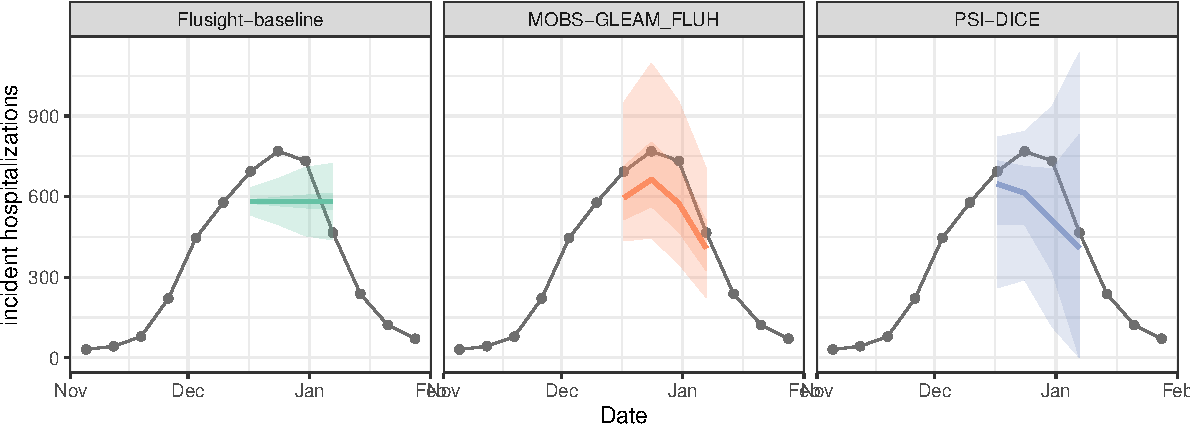
\includegraphics{hubEnsembles_manuscript_files/figure-pdf/fig-plot-ex-mods-1.pdf}

}

\caption{\label{fig-plot-ex-mods}One example set of quantile forecasts
for weekly incident influenza hospitalizations in Massachusetts from
each of three models (panels). Forecasts are represented by a median
(line), 50\% and 90\% prediction intervals (ribbons). Gray points
represent observed incident hospitalizations.}

\end{figure}%

Next, we examine the PMF forecasts for hospitalization intensity in the
example model output data. For this target, teams forecasted the
probability that hospitalization intensity will be ``low'',
``moderate'', ``high'', or ``very high''. These four categories are
determined by thresholds for weekly hospital admissions per 100,000
population. In other words, ``low'' hospitalization intensity in a given
week means few incident influenza hospitalizations per 100,000
population are predicted, whereas ``very high'' hospitalization
intensity means many hospitalizations per 100,000 population are
predicted. These forecasts are made for the same task ID variables as
the \texttt{quantile} forecasts of incident hospitalizations except for
the target, which is ``wk flu hosp rate category'' for these categorical
predictions.

\begin{longtable}[]{@{}
  >{\raggedright\arraybackslash}p{(\columnwidth - 10\tabcolsep) * \real{0.1935}}
  >{\raggedright\arraybackslash}p{(\columnwidth - 10\tabcolsep) * \real{0.2796}}
  >{\raggedleft\arraybackslash}p{(\columnwidth - 10\tabcolsep) * \real{0.1075}}
  >{\raggedright\arraybackslash}p{(\columnwidth - 10\tabcolsep) * \real{0.1505}}
  >{\raggedright\arraybackslash}p{(\columnwidth - 10\tabcolsep) * \real{0.1828}}
  >{\raggedleft\arraybackslash}p{(\columnwidth - 10\tabcolsep) * \real{0.0860}}@{}}

\caption{\label{tbl-example-forecasts-pmf}Example PMF model output for
forecasts of incident influenza hospitalization intensity. A subset of
predictions are shown: 1-week ahead PMF forecasts made on 2022-12-17 for
Massachusetts from three distinct models. We round the forecasted
probability (in the \texttt{value} column) to two digits. The
\texttt{location}, \texttt{reference\_date} and
\texttt{target\_end\_date} columns have been omitted for brevity. This
example data is provided in the \texttt{hubExamples} package.}

\tabularnewline

\toprule\noalign{}
\begin{minipage}[b]{\linewidth}\raggedright
\texttt{model\_id}
\end{minipage} & \begin{minipage}[b]{\linewidth}\raggedright
\texttt{target}
\end{minipage} & \begin{minipage}[b]{\linewidth}\raggedleft
\texttt{horizon}
\end{minipage} & \begin{minipage}[b]{\linewidth}\raggedright
\texttt{output\_type}
\end{minipage} & \begin{minipage}[b]{\linewidth}\raggedright
\texttt{output\_type\_id}
\end{minipage} & \begin{minipage}[b]{\linewidth}\raggedleft
\texttt{value}
\end{minipage} \\
\midrule\noalign{}
\endhead
\bottomrule\noalign{}
\endlastfoot
Flusight-baseline & wk flu hosp rate category & 1 & pmf & low & 0.000 \\
Flusight-baseline & wk flu hosp rate category & 1 & pmf & moderate &
0.003 \\
Flusight-baseline & wk flu hosp rate category & 1 & pmf & high &
0.073 \\
Flusight-baseline & wk flu hosp rate category & 1 & pmf & very high &
0.924 \\
MOBS-GLEAM\_FLUH & wk flu hosp rate category & 1 & pmf & low & 0.000 \\
MOBS-GLEAM\_FLUH & wk flu hosp rate category & 1 & pmf & moderate &
0.002 \\
MOBS-GLEAM\_FLUH & wk flu hosp rate category & 1 & pmf & high & 0.163 \\
MOBS-GLEAM\_FLUH & wk flu hosp rate category & 1 & pmf & very high &
0.835 \\
PSI-DICE & wk flu hosp rate category & 1 & pmf & low & 0.013 \\
PSI-DICE & wk flu hosp rate category & 1 & pmf & moderate & 0.065 \\
PSI-DICE & wk flu hosp rate category & 1 & pmf & high & 0.218 \\
PSI-DICE & wk flu hosp rate category & 1 & pmf & very high & 0.704 \\

\end{longtable}

We show a representative example of the hospitalization intensity
category forecasts in Table~\ref{tbl-example-forecasts-pmf}. Because
these forecasts are PMF output type, the \texttt{output\_type\_id}
column specifies the bin of hospitalization intensity and the
\texttt{value} column provides the forecasted probability of
hospitalization incidence being in that category. Values sum to 1 across
bins. For the MOBS-GLEAM\_FLUH and PSI-DICE models, incidence is
forecasted to decrease over the horizon (Figure~\ref{fig-plot-ex-mods}),
and correspondingly, there is lower probability of ``high'' and ``very
high'' hospitalization intensity for later horizons
(Figure~\ref{fig-plot-ex-mods-pmf}).

\begin{figure}

\centering{

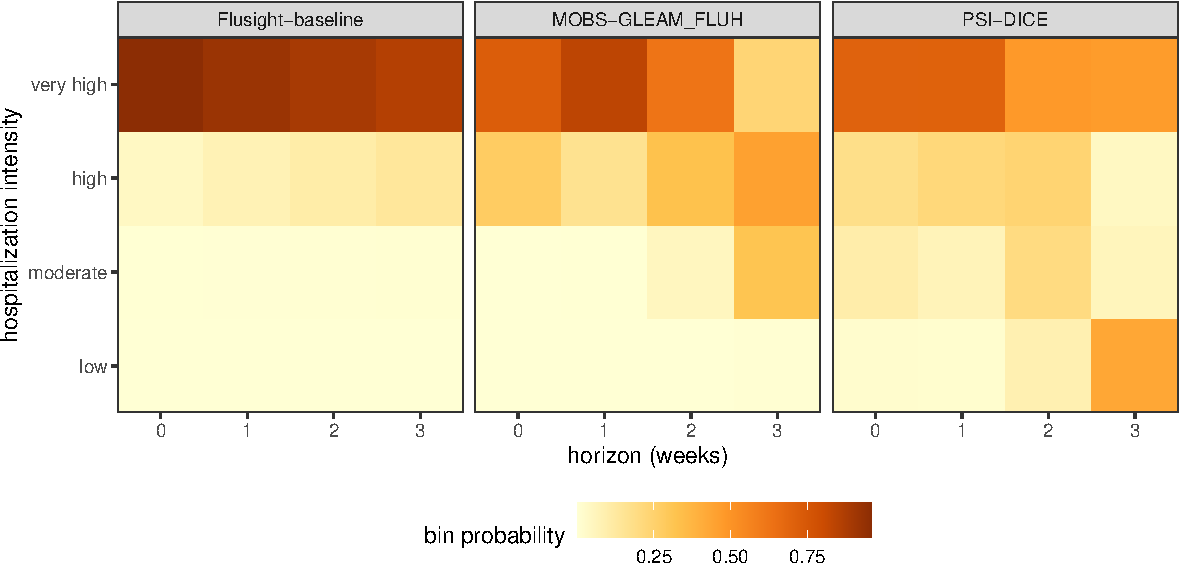
\includegraphics{hubEnsembles_manuscript_files/figure-pdf/fig-plot-ex-mods-pmf-1.pdf}

}

\caption{\label{fig-plot-ex-mods-pmf}One example PMF forecast of
incident influenza hospitalization intensity is shown for each of three
models (panels). Each cell shows the forecasted probability of a given
hospitalization intensity bin (low, moderate, high, and very high) for
each forecast horizon (0-3 weeks ahead). Darker colors indicate higher
forecasted probability.}

\end{figure}%

\subsection{Creating ensembles with
simple\_ensemble}\label{creating-ensembles-with-simple_ensemble}

Using the default options for \texttt{simple\_ensemble()}, we can
generate an equally weighted mean ensemble for each unique combination
of values for the task ID variables, the \texttt{output\_type} and the
\texttt{output\_type\_id}. Recall that this function corresponds to
different statistical ensemble methods for different output types: for
the quantile output type in our example data, the resulting ensemble is
a quantile average, while for the mean, median, CDF and PMF output
types, the ensemble is a linear pool.

\begin{Shaded}
\begin{Highlighting}[]
\SpecialCharTok{\textgreater{}}\NormalTok{ mean\_ens }\OtherTok{\textless{}{-}}\NormalTok{ hubExamples}\SpecialCharTok{::}\NormalTok{forecast\_outputs }\SpecialCharTok{|\textgreater{}}
\SpecialCharTok{+}\NormalTok{   dplyr}\SpecialCharTok{::}\FunctionTok{filter}\NormalTok{(output\_type }\SpecialCharTok{!=} \StringTok{"sample"}\NormalTok{) }\SpecialCharTok{|\textgreater{}}
\SpecialCharTok{+}\NormalTok{   hubEnsembles}\SpecialCharTok{::}\FunctionTok{simple\_ensemble}\NormalTok{(}
\SpecialCharTok{+}     \AttributeTok{model\_id =} \StringTok{"simple{-}ensemble{-}mean"}
\SpecialCharTok{+}\NormalTok{   )}
\end{Highlighting}
\end{Shaded}

The resulting model output has the same structure as the original model
output data (Table~\ref{tbl-mean-ensemble}), with columns for model ID,
task ID variables, output type, output type ID, and value. We also use
\texttt{model\_id\ =\ "simple-ensemble-mean"} to change the name of this
ensemble in the resulting model output; if not specified, the default is
``hub-ensemble''.

\begin{longtable}[]{@{}
  >{\raggedright\arraybackslash}p{(\columnwidth - 10\tabcolsep) * \real{0.2188}}
  >{\raggedright\arraybackslash}p{(\columnwidth - 10\tabcolsep) * \real{0.2708}}
  >{\raggedleft\arraybackslash}p{(\columnwidth - 10\tabcolsep) * \real{0.1042}}
  >{\raggedright\arraybackslash}p{(\columnwidth - 10\tabcolsep) * \real{0.1458}}
  >{\raggedright\arraybackslash}p{(\columnwidth - 10\tabcolsep) * \real{0.1771}}
  >{\raggedleft\arraybackslash}p{(\columnwidth - 10\tabcolsep) * \real{0.0833}}@{}}

\caption{\label{tbl-mean-ensemble}Mean ensemble model output. The values
in the \texttt{model\_id} column are set by the argument
\texttt{simple\_ensemble(...,\ model\_id)}. Results are generated for
all output types, but only a subset are shown: 1-week ahead forecasts
made on 2022-12-17 for Massachusetts, with only the median, 25th and
75th quantiles for the quantile output type and all bins for the PMF
output type. The \texttt{location}, \texttt{reference\_date} and
\texttt{target\_end\_date} columns have been omitted for brevity, and
the \texttt{value} column is rounded to two digits.}

\tabularnewline

\toprule\noalign{}
\begin{minipage}[b]{\linewidth}\raggedright
\texttt{model\_id}
\end{minipage} & \begin{minipage}[b]{\linewidth}\raggedright
\texttt{target}
\end{minipage} & \begin{minipage}[b]{\linewidth}\raggedleft
\texttt{horizon}
\end{minipage} & \begin{minipage}[b]{\linewidth}\raggedright
\texttt{output\_type}
\end{minipage} & \begin{minipage}[b]{\linewidth}\raggedright
\texttt{output\_type\_id}
\end{minipage} & \begin{minipage}[b]{\linewidth}\raggedleft
\texttt{value}
\end{minipage} \\
\midrule\noalign{}
\endhead
\bottomrule\noalign{}
\endlastfoot
simple-ensemble-mean & wk flu hosp rate category & 1 & pmf & high &
0.15 \\
simple-ensemble-mean & wk flu hosp rate category & 1 & pmf & low &
0.00 \\
simple-ensemble-mean & wk flu hosp rate category & 1 & pmf & moderate &
0.02 \\
simple-ensemble-mean & wk flu hosp rate category & 1 & pmf & very high &
0.82 \\
simple-ensemble-mean & wk inc flu hosp & 1 & mean & NA & 627.09 \\
simple-ensemble-mean & wk inc flu hosp & 1 & median & NA & 619.67 \\
simple-ensemble-mean & wk inc flu hosp & 1 & quantile & 0.25 & 541.67 \\
simple-ensemble-mean & wk inc flu hosp & 1 & quantile & 0.75 & 704.33 \\

\end{longtable}

\subsubsection{Changing the aggregation
function}\label{changing-the-aggregation-function}

We can change the function that is used to aggregate model outputs. For
example, we may want to calculate a median of the component models'
submitted values for each quantile. We do so by specifying
\texttt{agg\_fun\ =\ median}.

\begin{Shaded}
\begin{Highlighting}[]
\SpecialCharTok{\textgreater{}}\NormalTok{ median\_ens }\OtherTok{\textless{}{-}}\NormalTok{ hubExamples}\SpecialCharTok{::}\NormalTok{forecast\_outputs }\SpecialCharTok{|\textgreater{}}
\SpecialCharTok{+}\NormalTok{   dplyr}\SpecialCharTok{::}\FunctionTok{filter}\NormalTok{(output\_type }\SpecialCharTok{!=} \StringTok{"sample"}\NormalTok{) }\SpecialCharTok{|\textgreater{}}
\SpecialCharTok{+}\NormalTok{   hubEnsembles}\SpecialCharTok{::}\FunctionTok{simple\_ensemble}\NormalTok{(}
\SpecialCharTok{+}     \AttributeTok{agg\_fun =}\NormalTok{ median,}
\SpecialCharTok{+}     \AttributeTok{model\_id =} \StringTok{"simple{-}ensemble{-}median"}
\SpecialCharTok{+}\NormalTok{   )}
\end{Highlighting}
\end{Shaded}

Custom functions can also be passed into the \texttt{agg\_fun} argument.
We illustrate this by defining a custom function to compute the ensemble
prediction as a geometric mean of the component model predictions. Any
custom function to be used must have an argument \texttt{x} for the
vector of numeric values to summarize, and if relevant, an argument
\texttt{w} of numeric weights.

\begin{Shaded}
\begin{Highlighting}[]
\SpecialCharTok{\textgreater{}}\NormalTok{ geometric\_mean }\OtherTok{\textless{}{-}} \ControlFlowTok{function}\NormalTok{(x) \{}
\SpecialCharTok{+}\NormalTok{   n }\OtherTok{\textless{}{-}} \FunctionTok{length}\NormalTok{(x)}
\SpecialCharTok{+}   \FunctionTok{prod}\NormalTok{(x)}\SpecialCharTok{\^{}}\NormalTok{(}\DecValTok{1} \SpecialCharTok{/}\NormalTok{ n)}
\SpecialCharTok{+}\NormalTok{ \}}
\SpecialCharTok{\textgreater{}}\NormalTok{ geometric\_mean\_ens }\OtherTok{\textless{}{-}}\NormalTok{ hubExamples}\SpecialCharTok{::}\NormalTok{forecast\_outputs }\SpecialCharTok{|\textgreater{}}
\SpecialCharTok{+}\NormalTok{   dplyr}\SpecialCharTok{::}\FunctionTok{filter}\NormalTok{(output\_type }\SpecialCharTok{!=} \StringTok{"sample"}\NormalTok{) }\SpecialCharTok{|\textgreater{}}
\SpecialCharTok{+}\NormalTok{   hubEnsembles}\SpecialCharTok{::}\FunctionTok{simple\_ensemble}\NormalTok{(}
\SpecialCharTok{+}     \AttributeTok{agg\_fun =}\NormalTok{ geometric\_mean,}
\SpecialCharTok{+}     \AttributeTok{model\_id =} \StringTok{"simple{-}ensemble{-}geometric"}
\SpecialCharTok{+}\NormalTok{   )}
\end{Highlighting}
\end{Shaded}

As expected, the mean, median, and geometric mean each give us slightly
different resulting ensembles. The median point estimates, 50\%
prediction intervals, and 90\% prediction intervals in
Figure~\ref{fig-plot-ensembles} demonstrate this.

\begin{figure}

\centering{

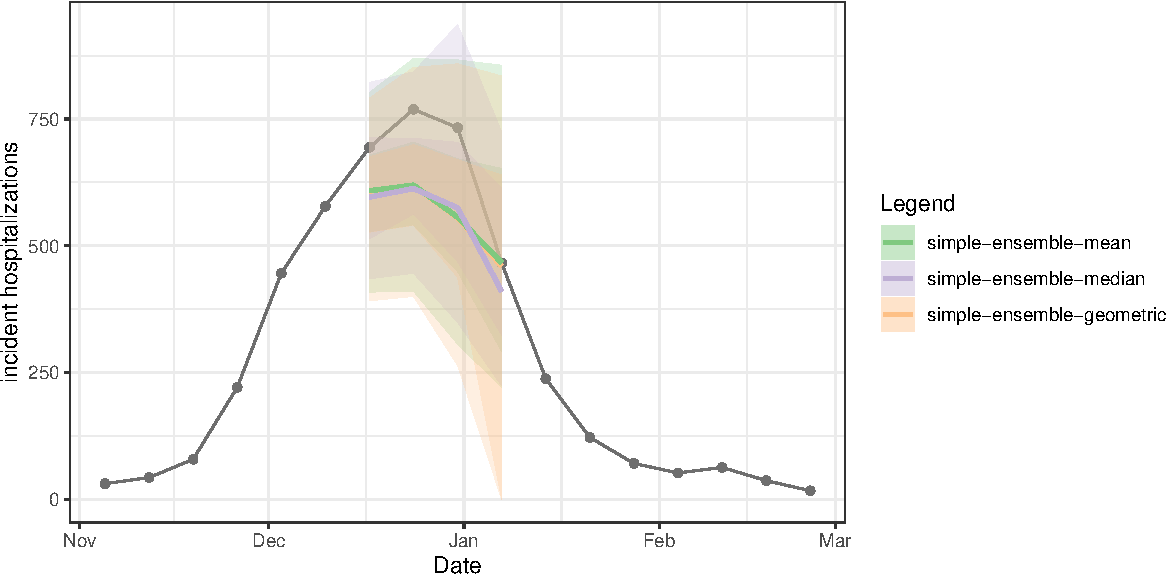
\includegraphics{hubEnsembles_manuscript_files/figure-pdf/fig-plot-ensembles-1.pdf}

}

\caption{\label{fig-plot-ensembles}Three different ensembles for weekly
incident influenza hospitalizations in Massachusetts. Each ensemble
combines individual predictions from the example hub
(Figure~\ref{fig-plot-ex-mods}) using a different method: arithmetic
mean, geometric mean, or median. All methods correspond to variations of
the quantile average approach. Ensembles are represented by a median
(line), 50\% and 90\% prediction intervals (ribbons). Geometric mean
ensemble and simple mean ensemble generate similar estimates in this
case.}

\end{figure}%

\subsubsection{Weighting model
contributions}\label{weighting-model-contributions}

We can weight the contributions of each model in the ensemble using the
\texttt{weights} argument of \texttt{simple\_ensemble()}. This argument
takes a \texttt{data.frame} that should include a \texttt{model\_id}
column containing each unique model ID and a \texttt{weight} column. In
the following example, we include the baseline model in the ensemble,
but give it less weight than the other forecasts.

\begin{Shaded}
\begin{Highlighting}[]
\SpecialCharTok{\textgreater{}}\NormalTok{ model\_weights }\OtherTok{\textless{}{-}} \FunctionTok{data.frame}\NormalTok{(}
\SpecialCharTok{+}   \AttributeTok{model\_id =} \FunctionTok{c}\NormalTok{(}\StringTok{"MOBS{-}GLEAM\_FLUH"}\NormalTok{, }\StringTok{"PSI{-}DICE"}\NormalTok{, }\StringTok{"Flusight{-}baseline"}\NormalTok{),}
\SpecialCharTok{+}   \AttributeTok{weight =} \FunctionTok{c}\NormalTok{(}\FloatTok{0.4}\NormalTok{, }\FloatTok{0.4}\NormalTok{, }\FloatTok{0.2}\NormalTok{)}
\SpecialCharTok{+}\NormalTok{ )}
\SpecialCharTok{\textgreater{}}\NormalTok{ weighted\_mean\_ens }\OtherTok{\textless{}{-}}\NormalTok{ hubExamples}\SpecialCharTok{::}\NormalTok{forecast\_outputs }\SpecialCharTok{|\textgreater{}}
\SpecialCharTok{+}\NormalTok{   dplyr}\SpecialCharTok{::}\FunctionTok{filter}\NormalTok{(output\_type }\SpecialCharTok{!=} \StringTok{"sample"}\NormalTok{) }\SpecialCharTok{|\textgreater{}}
\SpecialCharTok{+}\NormalTok{   hubEnsembles}\SpecialCharTok{::}\FunctionTok{simple\_ensemble}\NormalTok{(}
\SpecialCharTok{+}     \AttributeTok{weights =}\NormalTok{ model\_weights,}
\SpecialCharTok{+}     \AttributeTok{model\_id =} \StringTok{"simple{-}ensemble{-}weighted{-}mean"}
\SpecialCharTok{+}\NormalTok{   )}
\end{Highlighting}
\end{Shaded}

\subsection{Creating ensembles with
linear\_pool}\label{creating-ensembles-with-linear_pool}

We can also generate a linear pool ensemble, or distributional mixture,
using the \texttt{linear\_pool()} function; this function can be applied
to predictions with an \texttt{output\_type} of mean, quantile, sample,
CDF, or PMF. Our example hub includes the median output type, so we
exclude it from the calculation.

\begin{Shaded}
\begin{Highlighting}[]
\SpecialCharTok{\textgreater{}}\NormalTok{ linear\_pool\_ens }\OtherTok{\textless{}{-}}\NormalTok{ hubExamples}\SpecialCharTok{::}\NormalTok{forecast\_outputs }\SpecialCharTok{|\textgreater{}}
\SpecialCharTok{+}\NormalTok{   dplyr}\SpecialCharTok{::}\FunctionTok{filter}\NormalTok{(output\_type }\SpecialCharTok{!=} \StringTok{"median"}\NormalTok{) }\SpecialCharTok{|\textgreater{}}
\SpecialCharTok{+}\NormalTok{   hubEnsembles}\SpecialCharTok{::}\FunctionTok{linear\_pool}\NormalTok{(}\AttributeTok{model\_id =} \StringTok{"linear{-}pool"}\NormalTok{)}
\end{Highlighting}
\end{Shaded}

As described above, for \texttt{quantile} model outputs, the
\texttt{linear\_pool} function approximates the full probability
distribution for each component prediction using the value-quantile
pairs provided by that model, and then obtains quasi-random samples from
that distributional estimate. The number of samples drawn from the
distribution of each component model defaults to \texttt{1e4}, but this
can be changed using the \texttt{n\_samples} argument.

In Figure~\ref{fig-plot-ex-quantile-and-linear-pool}, we compare
ensemble results generated by \texttt{simple\_ensemble()} and
\texttt{linear\_pool()} for model outputs of output types PMF and
quantile. As expected, the results from the two functions are equivalent
for the PMF output type: for this output type, the
\texttt{simple\_ensemble()} method averages the predicted probability of
each category across the component models, which is the definition of
the linear pool ensemble method. This is not the case for the quantile
output type, because the \texttt{simple\_ensemble()} is computing a
quantile average.

\begin{figure}

\centering{

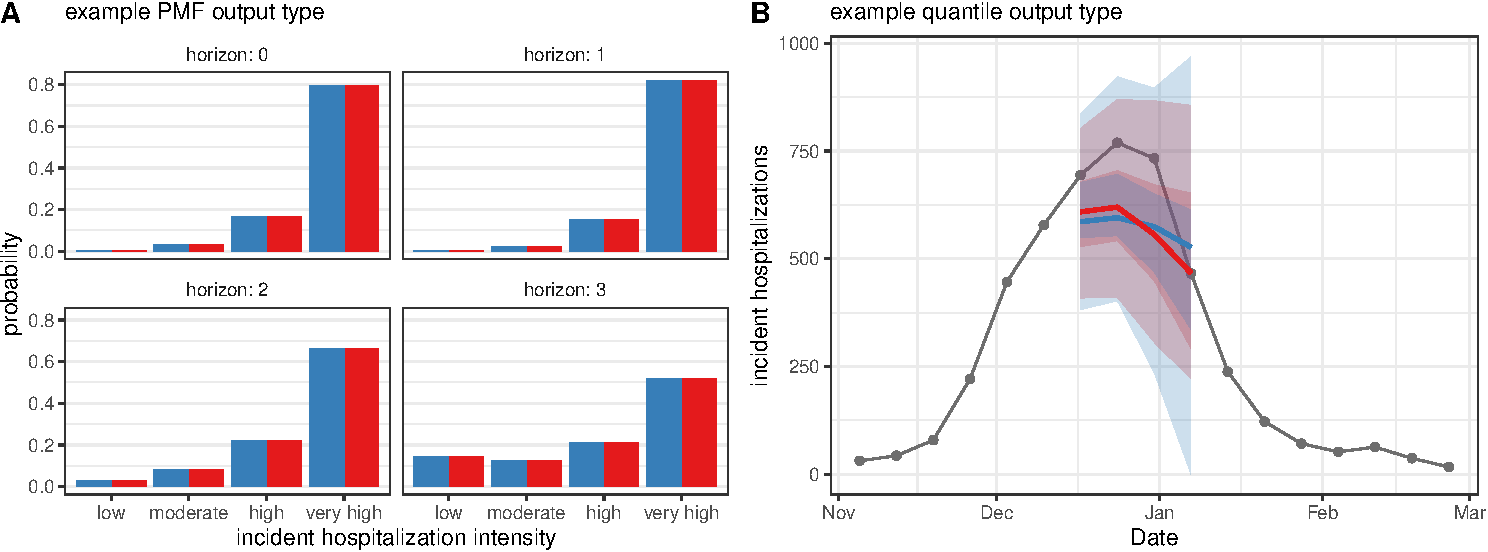
\includegraphics{hubEnsembles_manuscript_files/figure-pdf/fig-plot-ex-quantile-and-linear-pool-1.pdf}

}

\caption{\label{fig-plot-ex-quantile-and-linear-pool}Comparison of
results from \texttt{linear\_pool()} (blue) and
\texttt{simple\_ensemble()} (red). (Panel A) Ensemble predictions of
Massachusetts incident influenza hospitalization intensity (classified
as low, moderate, high, or very high), which provide an example of PMF
output type. (Panel B) Ensemble predictions of weekly incident influenza
hospitalizations in Massachusetts, which provide an example of quantile
output type. Note, for quantile output type, \texttt{simple\_ensemble()}
corresponds to a quantile average. Ensembles combine individual models
from the example hub, and are represented by a median (line), 50\% and
90\% prediction intervals (ribbons) (Figure~\ref{fig-plot-ex-mods}).}

\end{figure}%

\subsubsection{Weighting model
contributions}\label{weighting-model-contributions-1}

Like with \texttt{simple\_ensemble()}, we can change the default
function settings. For example, weights that determine a model's
contribution to the resulting ensemble may be provided. (Note that we
must exclude the sample output type here because it cannot yet be
combined into weighted ensembles.)

\begin{Shaded}
\begin{Highlighting}[]
\SpecialCharTok{\textgreater{}}\NormalTok{ weighted\_linear\_pool\_norm }\OtherTok{\textless{}{-}}\NormalTok{ hubExamples}\SpecialCharTok{::}\NormalTok{forecast\_outputs }\SpecialCharTok{|\textgreater{}}
\SpecialCharTok{+}\NormalTok{   dplyr}\SpecialCharTok{::}\FunctionTok{filter}\NormalTok{(}\SpecialCharTok{!}\NormalTok{output\_type }\SpecialCharTok{\%in\%} \FunctionTok{c}\NormalTok{(}\StringTok{"median"}\NormalTok{, }\StringTok{"sample"}\NormalTok{)) }\SpecialCharTok{|\textgreater{}}
\SpecialCharTok{+}\NormalTok{   hubEnsembles}\SpecialCharTok{::}\FunctionTok{linear\_pool}\NormalTok{(}
\SpecialCharTok{+}     \AttributeTok{weights =}\NormalTok{ model\_weights,}
\SpecialCharTok{+}     \AttributeTok{model\_id =} \StringTok{"linear{-}pool{-}weighted"}
\SpecialCharTok{+}\NormalTok{ )}
\end{Highlighting}
\end{Shaded}

\subsubsection{Changing the parametric family used for extrapolation
into distribution
tails}\label{changing-the-parametric-family-used-for-extrapolation-into-distribution-tails}

When requesting a linear pool of quantiles, we may also change the
distribution that \texttt{distfromq} uses to approximate the tails of
component models' predictive distributions to either log normal or
Cauchy using the \texttt{tail\_dist} argument (the default is
normal)\textsuperscript{47}. This choice usually does not have a large
impact on the resulting ensemble distribution, though, and can only be
seen in its outer edges. (For more details and other function options,
see the documentation in the \texttt{distfromq} package at
\url{https://reichlab.io/distfromq/}.)

\begin{Shaded}
\begin{Highlighting}[]
\SpecialCharTok{\textgreater{}}\NormalTok{ linear\_pool\_lnorm }\OtherTok{\textless{}{-}}\NormalTok{ hubExamples}\SpecialCharTok{::}\NormalTok{forecast\_outputs }\SpecialCharTok{|\textgreater{}}
\SpecialCharTok{+}\NormalTok{   dplyr}\SpecialCharTok{::}\FunctionTok{filter}\NormalTok{(output\_type }\SpecialCharTok{==} \StringTok{"quantile"}\NormalTok{) }\SpecialCharTok{|\textgreater{}}
\SpecialCharTok{+}\NormalTok{   hubEnsembles}\SpecialCharTok{::}\FunctionTok{linear\_pool}\NormalTok{(}
\SpecialCharTok{+}     \AttributeTok{model\_id =} \StringTok{"linear{-}pool{-}lognormal"}\NormalTok{,}
\SpecialCharTok{+}     \AttributeTok{tail\_dist =} \StringTok{"lnorm"}
\SpecialCharTok{+}\NormalTok{   )}
\SpecialCharTok{\textgreater{}}\NormalTok{ linear\_pool\_cauchy }\OtherTok{\textless{}{-}}\NormalTok{ hubExamples}\SpecialCharTok{::}\NormalTok{forecast\_outputs }\SpecialCharTok{|\textgreater{}}
\SpecialCharTok{+}\NormalTok{   dplyr}\SpecialCharTok{::}\FunctionTok{filter}\NormalTok{(output\_type }\SpecialCharTok{==} \StringTok{"quantile"}\NormalTok{) }\SpecialCharTok{|\textgreater{}}
\SpecialCharTok{+}\NormalTok{   hubEnsembles}\SpecialCharTok{::}\FunctionTok{linear\_pool}\NormalTok{(}
\SpecialCharTok{+}     \AttributeTok{model\_id =} \StringTok{"linear{-}pool{-}cauchy"}\NormalTok{,}
\SpecialCharTok{+}     \AttributeTok{tail\_dist =} \StringTok{"cauchy"}
\SpecialCharTok{+}\NormalTok{   )}
\end{Highlighting}
\end{Shaded}

\subsubsection{Requesting a subset of input sample predictions to be
ensembled}\label{requesting-a-subset-of-input-sample-predictions-to-be-ensembled}

Recall that for the sample output type, \texttt{linear\_pool()} defaults
to creating an equally-weighted ensemble by collecting and returning all
provided sample predictions, so that the total number of samples for the
ensemble is equal to the sum of the number of samples from all
individual models. To change this behavior, the user may instead specify
a number of sample predictions for the ensemble to return using the
\texttt{n\_output\_samples} argument. Then, a random subset of
predictions from individual models will be selected to construct a LOP
of samples so that all component models are represented equally. This
random selection of samples is stratified by model to ensure
approximately the same number of samples from each individual model is
included in the ensemble.

When requesting a linear pool composed of a subset of the input sample
predictions, the user must identify the task ID variables which together
identify a single modeled unit. This group of independent task ID
variables is called the compound task ID set and is specified using the
\texttt{compound\_taskid\_set} parameter to ensure the subsetting of
sample predictions is performed correctly. Samples summarizing a
marginal distribution will have a compound task ID set made up of all
the task ID variables. On the other hand, samples summarizing a joint
distribution will have a compound task ID set that contains only task ID
variables for which the joint distribution does not capture dependence.
For example, if a joint distribution is estimated across multiple
forecast horizons separately for each location, location would be
included in the compound task ID set but horizon would not.

Derived task IDs are another subgroup of task ID variables that must be
specified in a call to \texttt{linear\_pool()} for a subsetted sample
ensemble; their values are derived from a combination of the values from
other task ID variables (which may or may not be part of the compound
task ID set). A common example of a derived task ID variable is the
target date for a prediction, which is a deterministic function of the
reference date of the prediction and the prediction horizon. Generally,
the derived task IDs won't be included in the compound task ID set
because they are not needed to identify a single modeled unit for an
outcome of interest, \emph{unless} all of the task ID variables their
values depend on are already a part of the compound task ID set.

Not all model outputs will contain derived task IDs, in which case the
argument may be set to \texttt{NULL} (the default value). However, it is
important to provide the \texttt{linear\_pool()} function with any
derived task IDs when calculating an ensemble of (subsetted) samples, as
they are used to check that the provided compound task ID set is
compatible with the input predictions and the resulting LOP is valid.

\begin{Shaded}
\begin{Highlighting}[]
\SpecialCharTok{\textgreater{}}\NormalTok{ joint\_lp }\OtherTok{\textless{}{-}}\NormalTok{ hubExamples}\SpecialCharTok{::}\NormalTok{forecast\_outputs }\SpecialCharTok{|\textgreater{}}
\SpecialCharTok{+}\NormalTok{   dplyr}\SpecialCharTok{::}\FunctionTok{filter}\NormalTok{(output\_type }\SpecialCharTok{==} \StringTok{"sample"}\NormalTok{) }\SpecialCharTok{|\textgreater{}}
\SpecialCharTok{+}\NormalTok{   hubEnsembles}\SpecialCharTok{::}\FunctionTok{linear\_pool}\NormalTok{(}
\SpecialCharTok{+}     \AttributeTok{weights =} \ConstantTok{NULL}\NormalTok{,}
\SpecialCharTok{+}     \AttributeTok{model\_id =} \StringTok{"linear{-}pool{-}joint"}\NormalTok{,}
\SpecialCharTok{+}     \AttributeTok{task\_id\_cols =}
\SpecialCharTok{+}       \FunctionTok{c}\NormalTok{(}\StringTok{"reference\_date"}\NormalTok{, }\StringTok{"location"}\NormalTok{, }\StringTok{"horizon"}\NormalTok{, }\StringTok{"target"}\NormalTok{, }\StringTok{"target\_end\_date"}\NormalTok{),}
\SpecialCharTok{+}     \AttributeTok{compound\_taskid\_set =} \FunctionTok{c}\NormalTok{(}\StringTok{"reference\_date"}\NormalTok{, }\StringTok{"location"}\NormalTok{, }\StringTok{"target"}\NormalTok{),}
\SpecialCharTok{+}     \AttributeTok{derived\_tasks =} \StringTok{"target\_end\_date"}\NormalTok{,}
\SpecialCharTok{+}     \AttributeTok{n\_output\_samples =} \DecValTok{100}
\SpecialCharTok{+}\NormalTok{   )}
\end{Highlighting}
\end{Shaded}

\section{Example: in-depth analysis of forecast
data}\label{sec-case-study}

To further demonstrate the differences between the two ensemble
functions and the utility of the \texttt{hubEnsembles} package, we
provide a more complex example that walks through the full process of
generating multi-model ensembles. This case study gathers real forecasts
collected by a modeling hub to create four equally-weighted ensembles,
then evaluates their performance to determine the best approach for the
application.

The predictions we use to create the ensemble models are sourced from
two seasons of the FluSight forecasting challenge. Since 2013, the US
Centers for Disease Control and Prevention (CDC) has been soliciting
short-term forecasts of seasonal influenza from modeling teams through
this collaborative challenge\textsuperscript{49}. Using
\texttt{simple\_ensemble()} and \texttt{linear\_pool()}, we build four
equally-weighted, multi-model ensembles to predict weekly influenza
hospitalizations: a quantile (arithmetic) mean, a quantile median, a
linear pool with normal tails, and a linear pool with lognormal tails.
Then, we compare the resulting ensembles' performance through plotting
and scoring their forecasts.

Only a select portion of the code used in this analysis is shown for
brevity, but all the functions and scripts used to generate the case
study results can be found in the associated GitHub repository
(\url{https://github.com/hubverse-org/hubEnsemblesManuscript}). In
particular, the figures and tables supporting this analysis are
generated reproducibly using data from \texttt{.rds} files stored in the
\texttt{analysis/data/raw-data} directory and scripts in the
\texttt{inst} directory of the repository.

\subsection{Data and Methods}\label{data-and-methods}

We collect the predictions used to generate the four ensembles by
querying them from Zoltar\textsuperscript{50}, a repository designed to
archive forecasts created by the Reich Lab at UMass Amherst. For this
analysis we only consider FluSight forecasts in a quantile format from
the 2021-2022 and 2022-2023 influenza seasons. These quantile forecasts
are stored in two data objects, split by season, called
\texttt{flu\_forecasts-zoltar\_21-22.rds} and
\texttt{flu\_forecasts-zoltar\_22-23.rds}, which are then joined
together into a single data frame. A subset is shown below in
Table~\ref{tbl-raw-flu-forecasts}.

\begin{Shaded}
\begin{Highlighting}[]
\SpecialCharTok{\textgreater{}}\NormalTok{ flu\_forecasts\_raw\_21\_22 }\OtherTok{\textless{}{-}}\NormalTok{ readr}\SpecialCharTok{::}\FunctionTok{read\_rds}\NormalTok{(}
\SpecialCharTok{+}\NormalTok{   here}\SpecialCharTok{::}\FunctionTok{here}\NormalTok{(}\StringTok{"analysis/data/raw\_data/flu\_forecasts{-}zoltar\_21{-}22.rds"}\NormalTok{)}
\SpecialCharTok{+}\NormalTok{ )}
\SpecialCharTok{\textgreater{}}\NormalTok{ flu\_forecasts\_raw\_22\_23 }\OtherTok{\textless{}{-}}\NormalTok{ readr}\SpecialCharTok{::}\FunctionTok{read\_rds}\NormalTok{(}
\SpecialCharTok{+}\NormalTok{   here}\SpecialCharTok{::}\FunctionTok{here}\NormalTok{(}\StringTok{"analysis/data/raw\_data/flu\_forecasts{-}zoltar\_22{-}23.rds"}\NormalTok{)}
\SpecialCharTok{+}\NormalTok{ )}
\SpecialCharTok{\textgreater{}}\NormalTok{ flu\_forecasts\_raw }\OtherTok{\textless{}{-}} \FunctionTok{rbind}\NormalTok{(flu\_forecasts\_raw\_21\_22, flu\_forecasts\_raw\_22\_23)}
\end{Highlighting}
\end{Shaded}

\begin{longtable}[]{@{}
  >{\raggedright\arraybackslash}p{(\columnwidth - 16\tabcolsep) * \real{0.2095}}
  >{\raggedright\arraybackslash}p{(\columnwidth - 16\tabcolsep) * \real{0.2286}}
  >{\raggedright\arraybackslash}p{(\columnwidth - 16\tabcolsep) * \real{0.0857}}
  >{\raggedleft\arraybackslash}p{(\columnwidth - 16\tabcolsep) * \real{0.0762}}
  >{\raggedright\arraybackslash}p{(\columnwidth - 16\tabcolsep) * \real{0.0571}}
  >{\raggedright\arraybackslash}p{(\columnwidth - 16\tabcolsep) * \real{0.0667}}
  >{\raggedright\arraybackslash}p{(\columnwidth - 16\tabcolsep) * \real{0.0857}}
  >{\raggedleft\arraybackslash}p{(\columnwidth - 16\tabcolsep) * \real{0.1048}}
  >{\raggedright\arraybackslash}p{(\columnwidth - 16\tabcolsep) * \real{0.0857}}@{}}

\caption{\label{tbl-raw-flu-forecasts}An example prediction of weekly
incident influenza hospitalizations pulled directly from Zoltar. The
example forecasts were made on May 15, 2023 for California at the 1 week
ahead horizon. The forecasts were generated during the FluSight
forecasting challenge, then formatted according to Zoltar standards for
storage. The \texttt{timezero}, \texttt{season}, \texttt{unit},
\texttt{param1}, \texttt{param2}, and \texttt{param3} columns have been
omitted for brevity. (The \texttt{season} column has a value of
`2021-2022' or `2022-2023' while the last three `param' columns always
have a value of NA.)}

\tabularnewline

\toprule\noalign{}
\begin{minipage}[b]{\linewidth}\raggedright
\texttt{model}
\end{minipage} & \begin{minipage}[b]{\linewidth}\raggedright
\texttt{target}
\end{minipage} & \begin{minipage}[b]{\linewidth}\raggedright
\texttt{class}
\end{minipage} & \begin{minipage}[b]{\linewidth}\raggedleft
\texttt{value}
\end{minipage} & \begin{minipage}[b]{\linewidth}\raggedright
\texttt{cat}
\end{minipage} & \begin{minipage}[b]{\linewidth}\raggedright
\texttt{prob}
\end{minipage} & \begin{minipage}[b]{\linewidth}\raggedright
\texttt{sample}
\end{minipage} & \begin{minipage}[b]{\linewidth}\raggedleft
\texttt{quantile}
\end{minipage} & \begin{minipage}[b]{\linewidth}\raggedright
\texttt{family}
\end{minipage} \\
\midrule\noalign{}
\endhead
\bottomrule\noalign{}
\endlastfoot
UMass-trends\_ensemble & 1 wk ahead inc flu hosp & quantile & 12 & NA &
NA & NA & 0.025 & NA \\
UMass-trends\_ensemble & 1 wk ahead inc flu hosp & quantile & 17 & NA &
NA & NA & 0.100 & NA \\
UMass-trends\_ensemble & 1 wk ahead inc flu hosp & quantile & 25 & NA &
NA & NA & 0.250 & NA \\
UMass-trends\_ensemble & 1 wk ahead inc flu hosp & quantile & 46 & NA &
NA & NA & 0.750 & NA \\
UMass-trends\_ensemble & 1 wk ahead inc flu hosp & quantile & 56 & NA &
NA & NA & 0.900 & NA \\
UMass-trends\_ensemble & 1 wk ahead inc flu hosp & quantile & 68 & NA &
NA & NA & 0.975 & NA \\

\end{longtable}

Although these forecasts are in a tabular format, they are not
\texttt{model\_out\_tbl} objects and thus cannot yet be fed into either
of the \texttt{hubEnsembles} functions. Thus, we must use the
\texttt{as\_model\_out\_tbl()}\footnote{https://hubverse-org.github.io/hubUtils/reference/as\_model\_out\_tbl.html}
function from \texttt{hubUtils} to transform the raw forecasts so that
they conform to hubverse standards. Below, we specify the appropriate
column mappings in the call with task ID variables of
\texttt{forecast\_date} (when the forecast was made), \texttt{location},
\texttt{horizon}, and \texttt{target}.

\begin{Shaded}
\begin{Highlighting}[]
\SpecialCharTok{\textgreater{}}\NormalTok{ flu\_forecasts\_hubverse }\OtherTok{\textless{}{-}}\NormalTok{ flu\_forecasts\_raw }\SpecialCharTok{|\textgreater{}}
\SpecialCharTok{+}\NormalTok{   dplyr}\SpecialCharTok{::}\FunctionTok{rename}\NormalTok{(}\AttributeTok{forecast\_date =}\NormalTok{ timezero, }\AttributeTok{location =}\NormalTok{ unit) }\SpecialCharTok{|\textgreater{}}
\SpecialCharTok{+}\NormalTok{   tidyr}\SpecialCharTok{::}\FunctionTok{separate}\NormalTok{(target, }\AttributeTok{sep =} \StringTok{" "}\NormalTok{, }\AttributeTok{convert =} \ConstantTok{TRUE}\NormalTok{,}
\SpecialCharTok{+}                   \AttributeTok{into =} \FunctionTok{c}\NormalTok{(}\StringTok{"horizon"}\NormalTok{, }\StringTok{"target"}\NormalTok{), }\AttributeTok{extra =} \StringTok{"merge"}\NormalTok{) }\SpecialCharTok{|\textgreater{}}
\SpecialCharTok{+}\NormalTok{   dplyr}\SpecialCharTok{::}\FunctionTok{mutate}\NormalTok{(}\AttributeTok{target\_end\_date =} 
\SpecialCharTok{+}                   \FunctionTok{round\_date}\NormalTok{(forecast\_date }\SpecialCharTok{+} \FunctionTok{weeks}\NormalTok{(horizon), }\StringTok{"weeks"}\NormalTok{) }\SpecialCharTok{{-}}
\SpecialCharTok{+}                     \FunctionTok{days}\NormalTok{(}\DecValTok{1}\NormalTok{)) }\SpecialCharTok{|\textgreater{}}
\SpecialCharTok{+}   \FunctionTok{as\_model\_out\_tbl}\NormalTok{(}
\SpecialCharTok{+}     \AttributeTok{model\_id\_col =} \StringTok{"model"}\NormalTok{,}
\SpecialCharTok{+}     \AttributeTok{output\_type\_col =} \StringTok{"class"}\NormalTok{,}
\SpecialCharTok{+}     \AttributeTok{output\_type\_id\_col =} \StringTok{"quantile"}\NormalTok{,}
\SpecialCharTok{+}     \AttributeTok{value\_col =} \StringTok{"value"}\NormalTok{,}
\SpecialCharTok{+}     \AttributeTok{sep =} \StringTok{"{-}"}\NormalTok{,}
\SpecialCharTok{+}     \AttributeTok{trim\_to\_task\_ids =} \ConstantTok{FALSE}\NormalTok{,}
\SpecialCharTok{+}     \AttributeTok{hub\_con =} \ConstantTok{NULL}\NormalTok{,}
\SpecialCharTok{+}     \AttributeTok{task\_id\_cols =} 
\SpecialCharTok{+}       \FunctionTok{c}\NormalTok{(}\StringTok{"forecast\_date"}\NormalTok{, }\StringTok{"location"}\NormalTok{, }\StringTok{"horizon"}\NormalTok{, }\StringTok{"target"}\NormalTok{, target\_end\_date),}
\SpecialCharTok{+}     \AttributeTok{remove\_empty =} \ConstantTok{TRUE}
\SpecialCharTok{+}\NormalTok{   )}
\end{Highlighting}
\end{Shaded}

To ensure the quantile mean and median ensemble had consistent component
forecast make-up at every quantile level, we only included predictions
(defined by a unique combination of task ID variables) that contained
all 23 quantiles specified by FluSight
(\(\theta \in \{.010, 0.025, .050, .100, ..., .900, .950, .990\}\)).
This requirement required no further action on our part, since it was
consistent with FluSight submission guidelines. However, we did remove
the baseline and median ensemble models generated by the FluSight hub
from the component forecasts, a choice motivated by the desire to match
the composition of models in the official FluSight ensemble.

\begin{Shaded}
\begin{Highlighting}[]
\SpecialCharTok{\textgreater{}}\NormalTok{ flu\_forecasts\_component }\OtherTok{\textless{}{-}}\NormalTok{ dplyr}\SpecialCharTok{::}\FunctionTok{filter}\NormalTok{(}
\SpecialCharTok{+}\NormalTok{   flu\_forecasts\_hubverse,}
\SpecialCharTok{+}   \SpecialCharTok{!}\NormalTok{model\_id }\SpecialCharTok{\%in\%} \FunctionTok{c}\NormalTok{(}\StringTok{"Flusight{-}baseline"}\NormalTok{, }\StringTok{"Flusight{-}ensemble"}\NormalTok{)}
\SpecialCharTok{+}\NormalTok{ )}
\end{Highlighting}
\end{Shaded}

With these inclusion criteria, the final data set of component forecasts
consists of predictions from 25 modeling teams and 42 distinct models,
53 forecast dates (one per week), 54 US locations, 4 horizons, 1 target,
and 23 quantiles. In the 2021-2022 season, 25 models made predictions
for 22 weeks spanning from late January 2022 to late June 2022, and in
the 2022-2023 season, there were 31 models making predictions for 31
weeks spanning mid-October 2022 to mid-May 2023. Fourteen of the 42
total models made forecasts for both seasons. Locations consist of the
50 US states, Washington DC, Puerto Rico, the Virgin Islands, and the
entire US; horizons 1 to 4 weeks ahead, quantiles the 23 described
above, and target week ahead incident flu hospitalization. The values
for the forecasts are always non-negative. In
Table~\ref{tbl-case-study-flu-forecasts}, we provide an example of these
predictions, showing select quantiles from a single model, forecast
date, horizon, and location.

\begin{longtable}[]{@{}
  >{\raggedright\arraybackslash}p{(\columnwidth - 10\tabcolsep) * \real{0.2366}}
  >{\raggedright\arraybackslash}p{(\columnwidth - 10\tabcolsep) * \real{0.2366}}
  >{\raggedleft\arraybackslash}p{(\columnwidth - 10\tabcolsep) * \real{0.1075}}
  >{\raggedright\arraybackslash}p{(\columnwidth - 10\tabcolsep) * \real{0.1505}}
  >{\raggedleft\arraybackslash}p{(\columnwidth - 10\tabcolsep) * \real{0.1828}}
  >{\raggedleft\arraybackslash}p{(\columnwidth - 10\tabcolsep) * \real{0.0860}}@{}}

\caption{\label{tbl-case-study-flu-forecasts}An example prediction of
weekly incident influenza hospitalizations. The example model output was
made on May 15, 2023 for California at the 1 week ahead horizon. The
forecast was generated during the FluSight forecasting challenge, then
formatted according to hubverse standards post hoc. The
\texttt{location}, \texttt{forecast\_date}, and \texttt{season} columns
have been omitted for brevity; quantiles representing the endpoints of
the central 50\%, 80\% and 95\% prediction intervals are shown.}

\tabularnewline

\toprule\noalign{}
\begin{minipage}[b]{\linewidth}\raggedright
\texttt{model\_id}
\end{minipage} & \begin{minipage}[b]{\linewidth}\raggedright
\texttt{target}
\end{minipage} & \begin{minipage}[b]{\linewidth}\raggedleft
\texttt{horizon}
\end{minipage} & \begin{minipage}[b]{\linewidth}\raggedright
\texttt{output\_type}
\end{minipage} & \begin{minipage}[b]{\linewidth}\raggedleft
\texttt{output\_type\_id}
\end{minipage} & \begin{minipage}[b]{\linewidth}\raggedleft
\texttt{value}
\end{minipage} \\
\midrule\noalign{}
\endhead
\bottomrule\noalign{}
\endlastfoot
UMass-trends\_ensemble & wk ahead inc flu hosp & 1 & quantile & 0.025 &
12 \\
UMass-trends\_ensemble & wk ahead inc flu hosp & 1 & quantile & 0.100 &
17 \\
UMass-trends\_ensemble & wk ahead inc flu hosp & 1 & quantile & 0.250 &
25 \\
UMass-trends\_ensemble & wk ahead inc flu hosp & 1 & quantile & 0.750 &
46 \\
UMass-trends\_ensemble & wk ahead inc flu hosp & 1 & quantile & 0.900 &
56 \\
UMass-trends\_ensemble & wk ahead inc flu hosp & 1 & quantile & 0.975 &
68 \\

\end{longtable}

Next, we can combine the predictions into a single
\texttt{model\_out\_tbl} object used to generate forecasts for each
ensemble method. Then, we call the appropriate function
\texttt{hubEnsembles} to generate predictions for each equally-weighted
ensemble, storing the results in four separate objects of model output
data.

\begin{Shaded}
\begin{Highlighting}[]
\NormalTok{mean\_ensemble }\OtherTok{\textless{}{-}}\NormalTok{ hubEnsembles}\SpecialCharTok{::}\FunctionTok{simple\_ensemble}\NormalTok{(}
\NormalTok{  flu\_forecasts\_component,}
  \AttributeTok{weights =} \ConstantTok{NULL}\NormalTok{,}
  \AttributeTok{agg\_fun =}\NormalTok{ mean,}
  \AttributeTok{model\_id =} \StringTok{"mean{-}ensemble"}
\NormalTok{)}
\NormalTok{median\_ensemble }\OtherTok{\textless{}{-}}\NormalTok{ hubEnsembles}\SpecialCharTok{::}\FunctionTok{simple\_ensemble}\NormalTok{(}
\NormalTok{  flu\_forecasts\_component,}
    \AttributeTok{weights =} \ConstantTok{NULL}\NormalTok{,}
    \AttributeTok{agg\_fun =}\NormalTok{ median,}
    \AttributeTok{model\_id =} \StringTok{"median{-}ensemble"}
\NormalTok{  )}
\NormalTok{lp\_normal }\OtherTok{\textless{}{-}}\NormalTok{ hubEnsembles}\SpecialCharTok{::}\FunctionTok{linear\_pool}\NormalTok{(}
\NormalTok{  flu\_forecasts\_component,}
  \AttributeTok{weights =} \ConstantTok{NULL}\NormalTok{,}
  \AttributeTok{n\_samples =} \FloatTok{1e5}\NormalTok{,}
  \AttributeTok{model\_id =} \StringTok{"lp{-}normal"}\NormalTok{,}
  \AttributeTok{tail\_dist =} \StringTok{"norm"}
\NormalTok{)}
\NormalTok{lp\_lognormal }\OtherTok{\textless{}{-}}\NormalTok{ hubEnsembles}\SpecialCharTok{::}\FunctionTok{linear\_pool}\NormalTok{(}
\NormalTok{  flu\_forecasts\_component,}
  \AttributeTok{weights =} \ConstantTok{NULL}\NormalTok{,}
  \AttributeTok{n\_samples =} \FloatTok{1e5}\NormalTok{,}
  \AttributeTok{model\_id =} \StringTok{"lp{-}lognormal"}\NormalTok{,}
  \AttributeTok{tail\_dist =} \StringTok{"lnorm"}
\NormalTok{) }
\end{Highlighting}
\end{Shaded}

We then evaluate the performance of the ensembles using scoring metrics
that measure the accuracy and calibration of their forecasts. We chose
several common metrics in forecast evaluation, including mean absolute
error (MAE), weighted interval score (WIS)\textsuperscript{51}, 50\%
prediction interval (PI) coverage, and 95\% PI coverage. MAE measures
the average absolute error of a set of point forecasts; smaller values
of MAE indicate better forecast accuracy. WIS is a generalization of MAE
for probabilistic forecasts and is an alternative to other common proper
scoring rules which cannot be evaluated directly for quantile
forecasts\textsuperscript{51}. WIS is made up of three component
penalties: (1) for over-prediction, (2) for under-prediction, and (3)
for the spread of each interval (where an interval is defined by a
symmetric set of two quantiles). This metric is a weighted sum of these
penalties across all prediction intervals provided. A lower WIS value
indicates a more accurate forecast\textsuperscript{51}. PI coverage
provides information about whether a forecast has accurately
characterized its uncertainty about future observations. The \(50\)\% PI
coverage rate measures the proportion of the time that 50\% prediction
intervals at that nominal level included the observed value; the 95\% PI
coverage rate is defined similarly. Achieving approximately nominal
(50\% or 95\%) coverage indicates a well-calibrated forecast.

We also use relative versions of WIS and MAE (rWIS and rMAE,
respectively) to understand how the ensemble performance compares to
that of the FluSight baseline model. These metrics are calculated as
\[\textrm{rWIS} = \frac{\textrm{WIS}_{\textrm{model }m}}{\textrm{WIS}_{\textrm{baseline}}} \hspace{3cm} \textrm{rMAE} = \frac{\textrm{MAE}_{\textrm{model }m}}{\textrm{MAE}_{\textrm{baseline}}},\]
where model \(m\) is any given model being compared against the
baseline. For both of these metrics, a value less than one indicates
better performance compared to the baseline while a value greater than
one indicates worse performance. By definition, the FluSight baseline
itself will always have a value of one for both of these metrics.

Each unique prediction from an ensemble model is scored against target
data using the \texttt{score\_forecasts()}\footnote{https://reichlab.io/covidHubUtils/reference/score\_forecasts.html}
function from the \texttt{covidHubUtils} package, made for scoring
tabular infectious disease data with commonly used evaluation metrics
including those mentioned above. We use median forecasts taken from the
0.5 quantile for the MAE evaluation.

\subsection{Performance results across
ensembles}\label{performance-results-across-ensembles}

The quantile median ensemble has the best overall performance in terms
of WIS and MAE (and the relative versions of these metrics), and has
coverage rates that were close to the nominal levels
(Table~\ref{tbl-overall-evaluation}). The two linear opinion pools have
very similar performance to each other. These methods have the
second-best performance as measured by WIS and MAE, but they have the
highest 50\% and 95\% coverage rates, with empirical coverage that was
well above the nominal coverage rate. The quantile mean performs the
worst of the ensembles with the highest MAE, which is substantially
different from that of the other ensembles.

\begin{longtable}[]{@{}lrrrrrr@{}}

\caption{\label{tbl-overall-evaluation}Summary of overall model
performance across both seasons, averaged over all locations except the
US national location and sorted by ascending WIS. The quantile median
ensemble has the best value for every metric except 50\% coverage rate,
though metric values are often quite similar among the models.}

\tabularnewline

\toprule\noalign{}
\texttt{model} & \texttt{wis} & \texttt{rwis} & \texttt{mae} &
\texttt{rmae} & \texttt{cov50} & \texttt{cov95} \\
\midrule\noalign{}
\endhead
\bottomrule\noalign{}
\endlastfoot
median-ensemble & 18.158 & 0.794 & 27.360 & 0.933 & 0.597 & 0.922 \\
lp-normal & 19.745 & 0.863 & 27.932 & 0.953 & 0.709 & 0.990 \\
lp-lognormal & 19.747 & 0.863 & 27.933 & 0.953 & 0.708 & 0.990 \\
mean-ensemble & 20.180 & 0.882 & 29.582 & 1.009 & 0.595 & 0.889 \\
Flusight-baseline & 22.876 & 1.000 & 29.315 & 1.000 & 0.604 & 0.881 \\

\end{longtable}

Plots of the models' forecasts can aid our understanding about the
origin of these accuracy differences. For example, the linear opinion
pools consistently have some of the widest prediction intervals, and
consequently the highest coverage rates. The median ensemble, which has
the best WIS, balanced interval width with calibration best overall,
with narrower intervals than the linear pools that still achieved
near-nominal coverage on average across all time points. The quantile
mean's interval widths vary, though it usually has narrower intervals
than the linear pools. However, this model's point forecasts have a
larger error margin compared to the other ensembles, especially at
longer horizons. This pattern is demonstrated in
Figure~\ref{fig-plot-forecasts-hubVis} for the 4-week ahead forecast in
California following the 2022-23 season peak on December 5, 2022. Here,
the quantile mean predicted a continued increase in hospitalizations, at
a steeper slope than the other ensemble methods.

\begin{figure}

\centering{

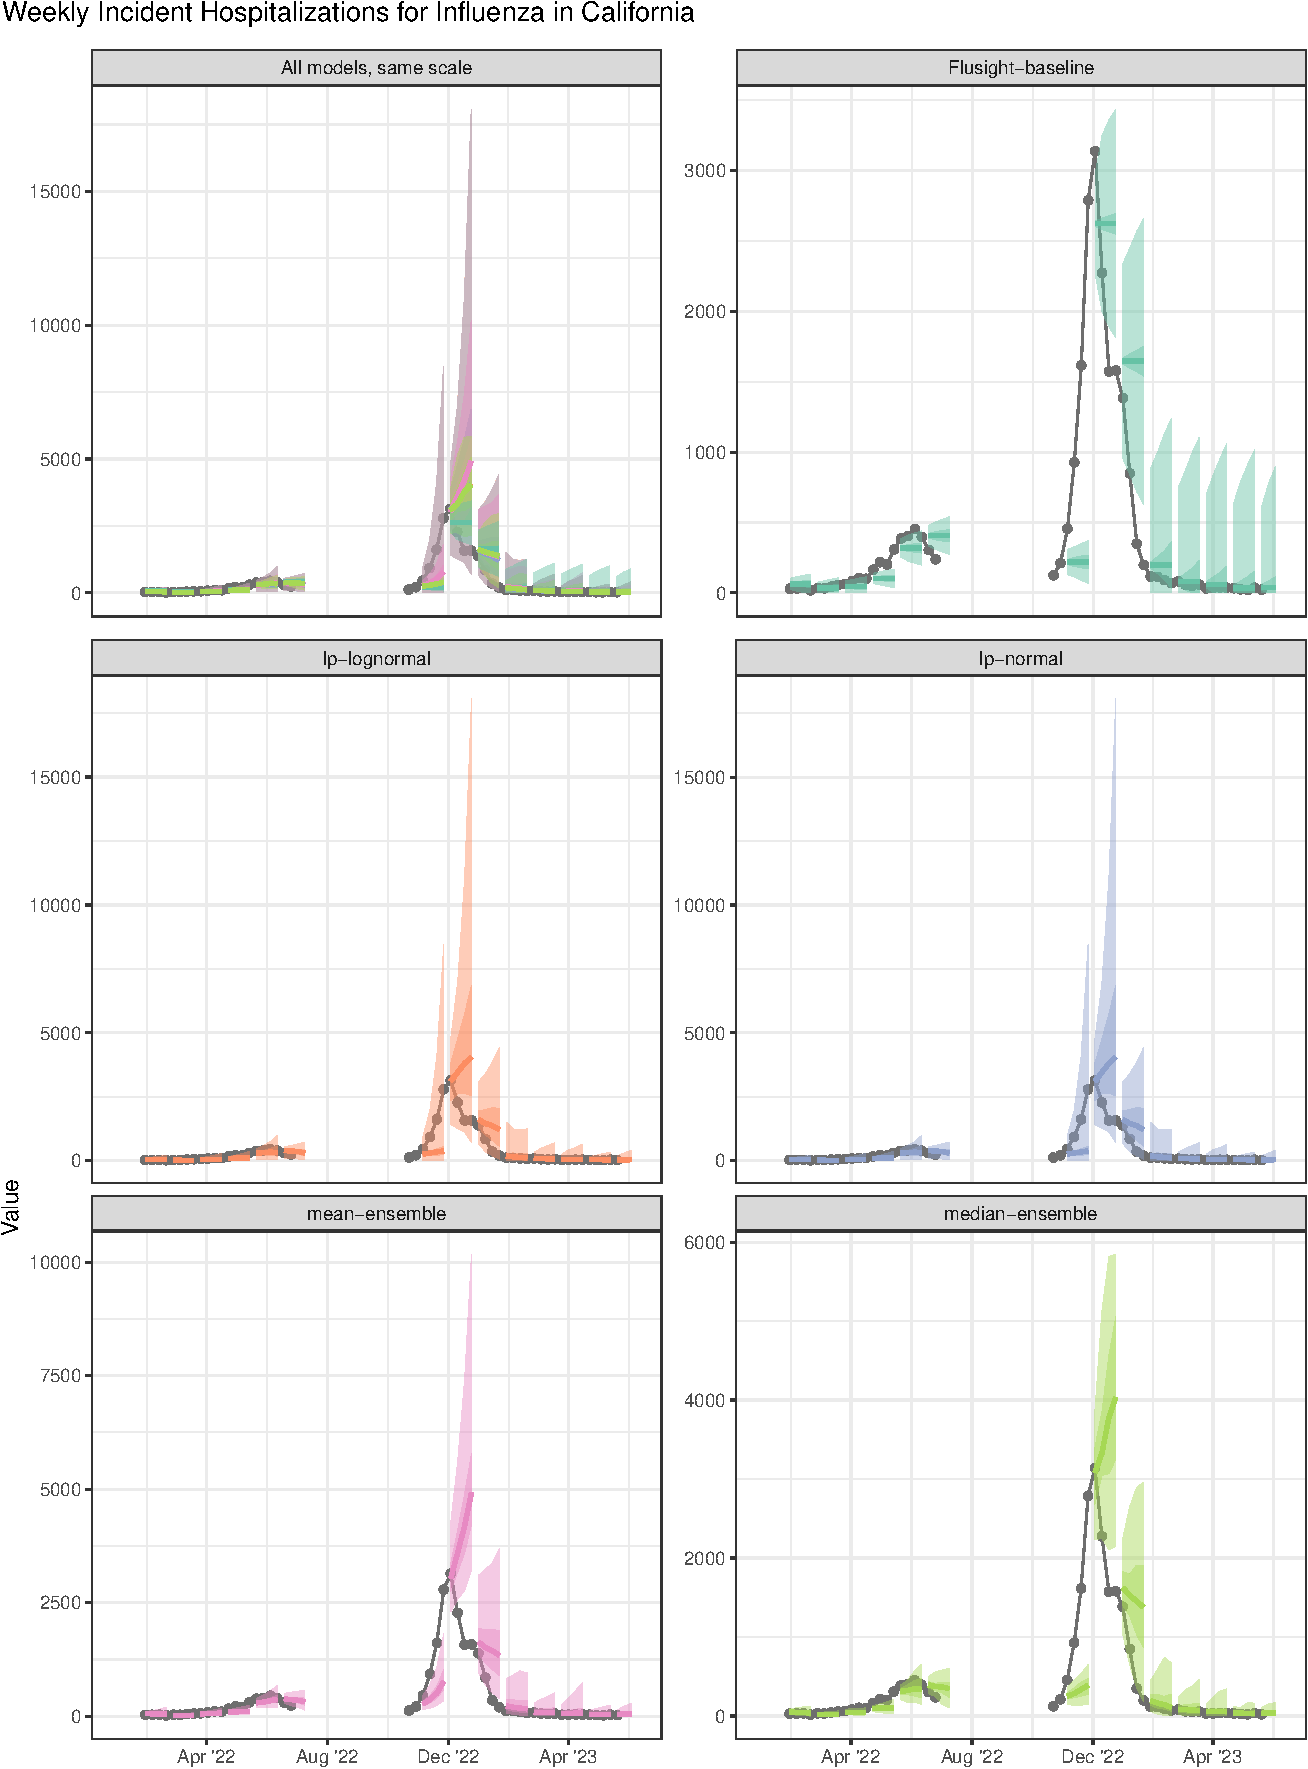
\includegraphics{hubEnsembles_manuscript_files/figure-pdf/fig-plot-forecasts-hubVis-1.pdf}

}

\caption{\label{fig-plot-forecasts-hubVis}One to four week ahead
forecasts for select dates plotted against target data for California.
The first panel shows all models on the same scale. All other panels
show forecasts for each individual model, with varying y-axis scales,
and their prediction accuracy as compared to observed influenza
hospitalizations.}

\end{figure}%

Averaging across all time points, the median ensemble has the best
scores for every metric. (Note that we only show plots of WIS vs
forecast date, faceted by season and horizon, due to similar trends
being observed with MAE and 95\% prediction interval coverage). The
quantile median outperforms the mean ensemble by a similar amount for
both WIS and MAE, particularly around local times of change (see
Figure~\ref{fig-wis-vs-forecast-date}). The median ensemble also has
better coverage rates than the mean ensemble in the tails of the
distribution (95\% intervals) and similar coverage in the center (50\%
intervals). The median model also outperforms the linear pools for most
weeks, with the greatest differences in scores being for WIS and
coverage rates (Figure~\ref{fig-wis-vs-forecast-date}). This seems to
indicate that the linear pools' estimates are usually too conservative,
with their wide intervals and higher-than-nominal coverage rates being
penalized by WIS. However, during the 2022-2023 season there are several
localized times when the linear pools showcased better one-week-ahead
forecasts than the median ensemble
(Figure~\ref{fig-wis-vs-forecast-date}). These localized instances are
characterized by similar MAE values for the two methods and poor median
ensemble coverage rates. In these instances, the wide intervals from the
linear pools were useful in capturing the eventually-observed
hospitalizations, usually during times of rapid change.

\begin{figure}

\centering{

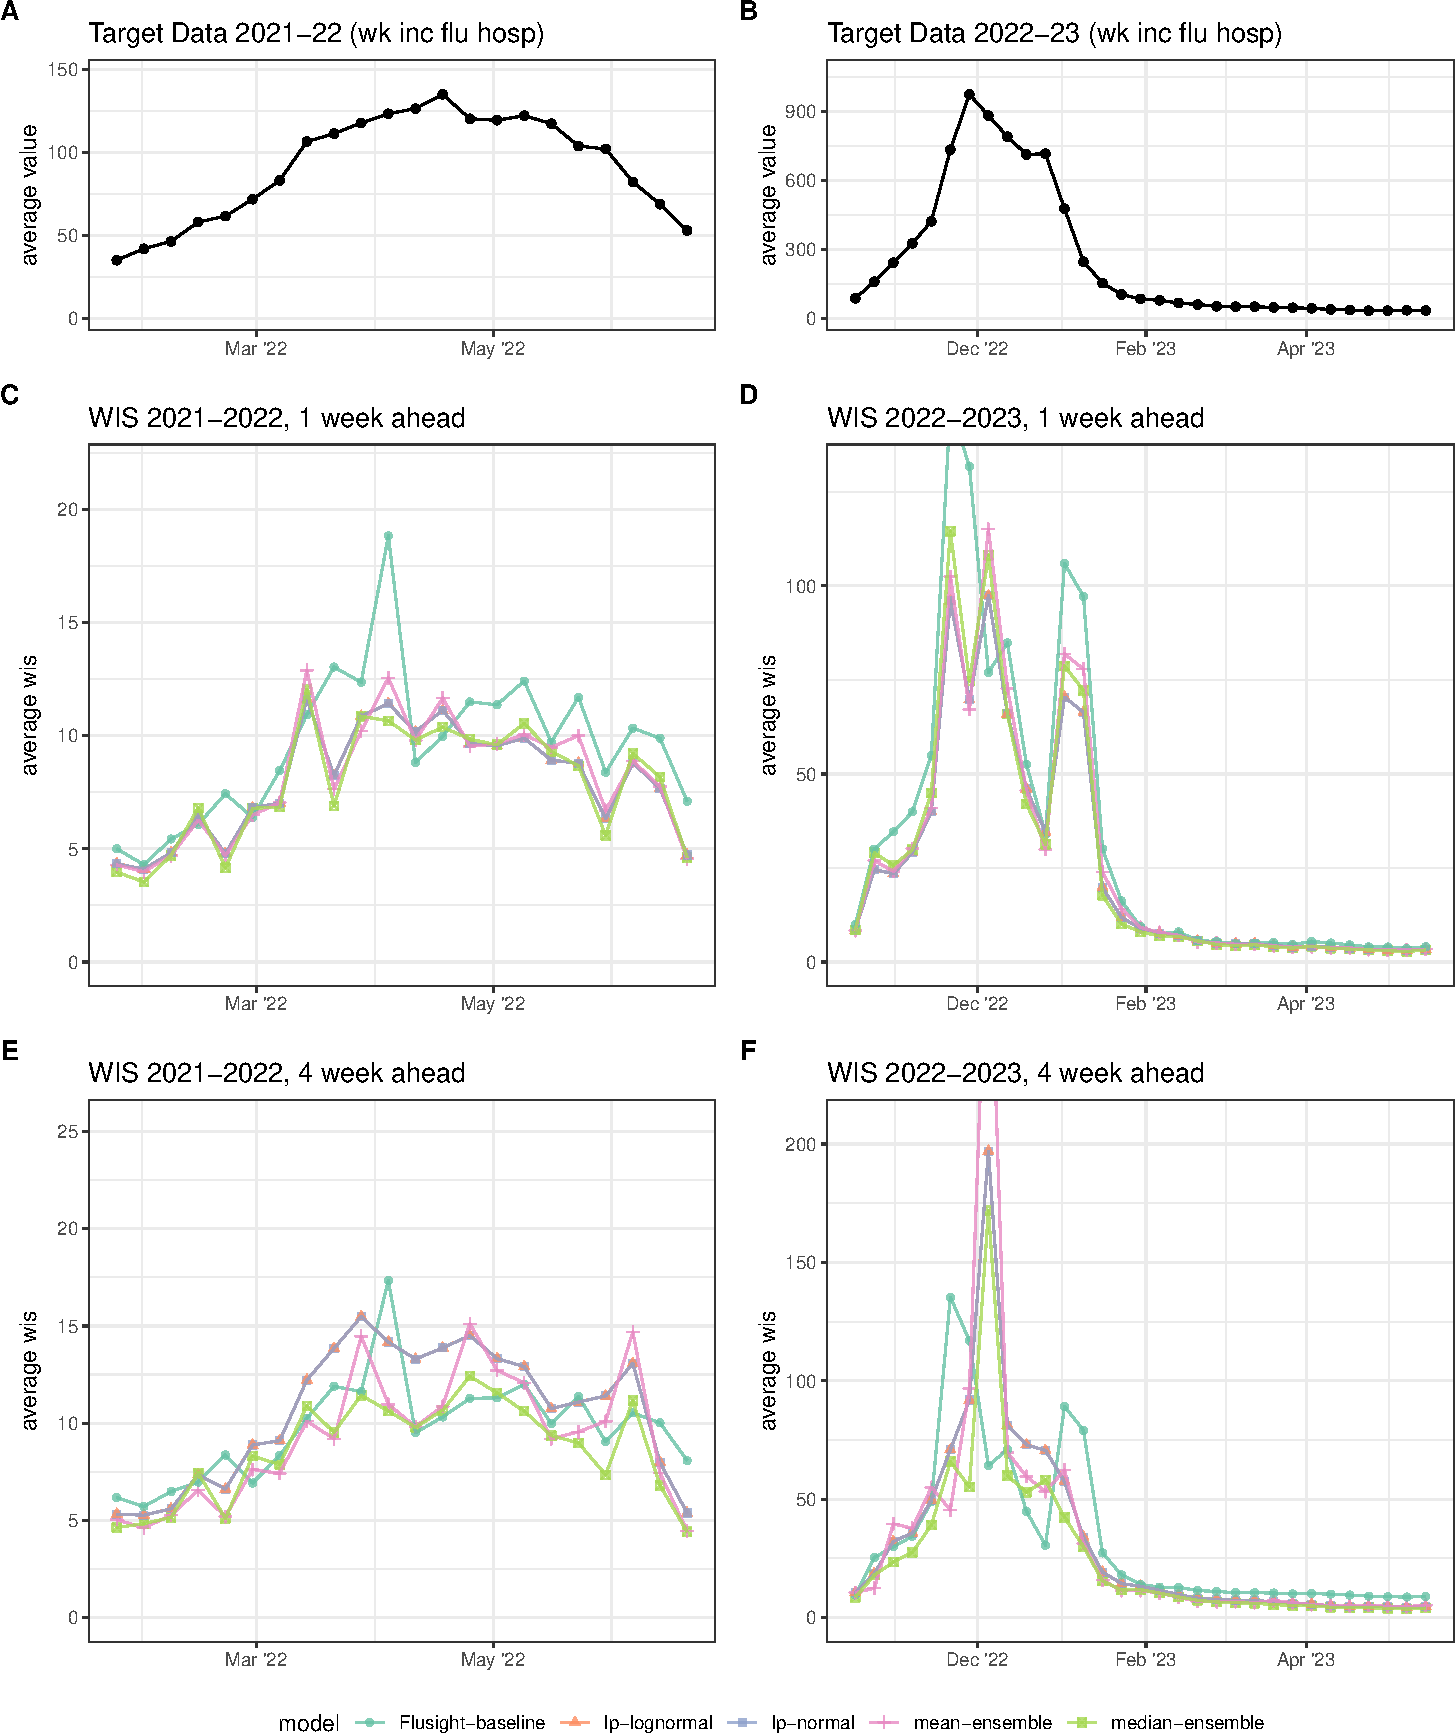
\includegraphics{hubEnsembles_manuscript_files/figure-pdf/fig-wis-vs-forecast-date-1.pdf}

}

\caption{\label{fig-wis-vs-forecast-date}Weighted interval score (WIS)
averaged across all locations. Average target data across all locations
for 2021-2022 (A) and 2022-2023 (B) seasons for reference. For each
season, average WIS is shown for 1-week (C-D) and 4-week ahead (E-F)
forecasts. Results are plotted for each ensemble model (colors) across
the entire season. Lower values indicate better performance.}

\end{figure}%

All of the ensemble variations outperform the baseline model in this
analysis, led by the quantile median which had the best scores overall
for WIS, MAE, 50\% PI coverage, and 95\% PI coverage. However, other
models sometimes demonstrated better performance, especially around the
season's peak. These results seem to be consistent with previous
findings: linear pools produce intervals generally too wide for a
short-term forecasting, except under conditions with greater levels of
uncertainty or where the individual models contributing to the ensemble
are poorly calibrated. Thus, while the quantile median offers
consistency and robustness, there may be certain influenza seasons in
which other ensemble methods display better performance.

The choice of an appropriate ensemble aggregation method may depend on
the forecast target, the goal of forecasting, and the behavior of the
individual models contributing to an ensemble. One case may call for
prioritizing high coverage rates while another may prioritize accurate
point forecasts. The \texttt{simple\_ensemble()} and
\texttt{linear\_pool()} functions and the ability to specify component
model weights and an aggregation function for
\texttt{simple\_ensemble()} allow users to implement a variety of
ensemble methods.

\section{Summary and discussion}\label{sec-conclusions}

Ensembles of independent models are a powerful tool to generate more
accurate and more reliable predictions of future outcomes than a single
model alone. Here, we have provided an overview of multi-model ensemble
methodology with the goal of improving use of ensemble results in public
health and biomedical research settings, as well as other domains that
use probabilistic forecasting. Moreover, we have demonstrated how to
utilize \texttt{hubEnsembles}, a simple and flexible framework to
combine individual model predictions into an ensemble.

Multi-model ensembles are becoming the gold standard for prediction
exercises in the public health domain. Collaborative modeling hubs can
serve as a centralized entity to guide and elicit predictions from
multiple independent models, as well as to generate and communicate
ensemble results\textsuperscript{12,36}. Given the increasing popularity
of multi-model ensembles and collaborative hubs, there is a clear need
for generalized data standards and software infrastructure to support
these hubs. By addressing this need, the hubverse suite of tools can
reduce duplicative efforts across existing hubs, support other
communities engaged in collaborative efforts, and enable the adoption of
multi-model approaches in new domains.

When generating and interpreting an ensemble prediction, it is important
to understand the methods underlying the ensemble, as methodological
choices can have meaningful effects on the resulting ensemble and its
performance. Although there may not be a universal ``best'' method,
matching the properties of a given ensemble method with the features of
the component models will likely yield best results\textsuperscript{24}.
Our case study on seasonal influenza forecasts in the US demonstrates
this point. The quantile median ensemble performs best overall for a
range of metrics, including weighted interval score, mean absolute
error, and prediction interval coverage. Yet, the other ensemble methods
we tested also showcased a clear improvement over the baseline model and
even outperformed the quantile median for certain weeks, particularly
during periods of rapid change when outlying component forecasts are
likely more important. The accuracy gains from ensemble models motivate
the use of a ``hub-based'' approach to prediction for infectious
diseases, public health, and in other fields.

\section*{Acknowledgements}\label{acknowledgements}
\addcontentsline{toc}{section}{Acknowledgements}

The authors thank all members of the hubverse community; the broader
hubverse software infrastructure made this package possible. L.
Shandross, A. Krystalli, N. G. Reich, and E. L. Ray were supported by
the National Institutes of General Medical Sciences (R35GM119582) and
the US Centers for Disease Control and Prevention (U01IP001122 and
NU38FT000008). E. Howerton was supported by NSF RAPID awards DEB-2126278
and DEB-2220903, as well as the Eberly College of Science Barbara
McClintock Science Achievement Graduate Scholarship in Biology at the
Pennsylvania State University. L. Contamin and H. Hochheiser were
supported by NIGMS grants U24GM132013 and R24GM153920. The content is
solely the responsibility of the authors and does not necessarily
represent the official views of NIGMS, the National Institutes of
Health, or CDC.

\section*{Consortium of Infectious Disease Modeling
Hubs}\label{consortium-of-infectious-disease-modeling-hubs}
\addcontentsline{toc}{section}{Consortium of Infectious Disease Modeling
Hubs}

Consortium of Infectious Disease Modeling Hubs authors include Alvaro J.
Castro Rivadeneira (University of Massachusetts Amherst), Lucie Contamin
(University of Pittsburgh), Sebastian Funk (London School of Hygiene \&
Tropical Medicine), Aaron Gerding (University of Massachusetts Amherst),
Hugo Gruson (data.org), Harry Hochheiser (University of Pittsburgh),
Emily Howerton (The Pennsylvania State University), Melissa Kerr
(University of Massachusetts Amherst), Anna Krystalli (R-RSE SMPC), Sara
L. Loo (Johns Hopkins University), Evan L. Ray (University of
Massachusetts Amherst), Nicholas G. Reich (University of Massachusetts
Amherst), Koji Sato (Johns Hopkins University), Li Shandross (University
of Massachusetts Amherst), Katharine Sherratt (London School of Hygene
and Tropical Medicine), Shaun Truelove (Johns Hopkins University),
Martha Zorn (University of Massachusetts Amherst)

\section*{References}\label{references}
\addcontentsline{toc}{section}{References}

\phantomsection\label{refs}
\begin{CSLReferences}{0}{1}
\bibitem[\citeproctext]{ref-clemen1989}
\CSLLeftMargin{1. }%
\CSLRightInline{Clemen RT. Combining forecasts: A review and annotated
bibliography. \emph{International Journal of Forecasting}.
1989;5(4):559-583.
doi:\href{https://doi.org/10.1016/0169-2070(89)90012-5}{10.1016/0169-2070(89)90012-5}}

\bibitem[\citeproctext]{ref-timmermann2006}
\CSLLeftMargin{2. }%
\CSLRightInline{Timmermann A. Chapter 4 Forecast Combinations. In: Vol
1. Elsevier; 2006:135-196.
doi:\href{https://doi.org/10.1016/S1574-0706(05)01004-9}{10.1016/S1574-0706(05)01004-9}}

\bibitem[\citeproctext]{ref-hibon2005}
\CSLLeftMargin{3. }%
\CSLRightInline{Hibon M, Evgeniou T. To combine or not to combine:
selecting among forecasts and their combinations. \emph{International
Journal of Forecasting}. 2005;21(1):15-24.
doi:\href{https://doi.org/10.1016/j.ijforecast.2004.05.002}{10.1016/j.ijforecast.2004.05.002}}

\bibitem[\citeproctext]{ref-alley2019}
\CSLLeftMargin{4. }%
\CSLRightInline{Alley RB, Emanuel KA, Zhang F. Advances in weather
prediction. \emph{Science}. 2019;363(6425):342-344.
doi:\href{https://doi.org/10.1126/science.aav7274}{10.1126/science.aav7274}}

\bibitem[\citeproctext]{ref-tebaldi2007}
\CSLLeftMargin{5. }%
\CSLRightInline{Tebaldi C, Knutti R. The use of the multi-model ensemble
in probabilistic climate projections. \emph{Philosophical Transactions:
Mathematical, Physical and Engineering Sciences}.
2007;365(1857):2053-2075.
doi:\href{https://doi.org/10.1098/rsta.2007.2076}{10.1098/rsta.2007.2076}}

\bibitem[\citeproctext]{ref-aastveit2018}
\CSLLeftMargin{6. }%
\CSLRightInline{Aastveit KA, Mitchell J, Ravazzolo F, Dijk HK van. The
Evolution of Forecast Density Combinations in Economics. \emph{Tinbergen
Institute Discussion Papers}. Published online 2018.
\url{https://hdl.handle.net/10419/185588}}

\bibitem[\citeproctext]{ref-shaman_improved_2015}
\CSLLeftMargin{7. }%
\CSLRightInline{Shaman J, Kandula S. Improved {Discrimination} of
{Influenza} {Forecast} {Accuracy} {Using} {Consecutive} {Predictions}.
\emph{PLoS Currents}.
2015;7:ecurrents.outbreaks.8a6a3df285af7ca973fab4b22e10911e.
doi:\href{https://doi.org/10.1371/currents.outbreaks.8a6a3df285af7ca973fab4b22e10911e}{10.1371/currents.outbreaks.8a6a3df285af7ca973fab4b22e10911e}}

\bibitem[\citeproctext]{ref-held_probabilistic_2017}
\CSLLeftMargin{8. }%
\CSLRightInline{Held L, Meyer S, Bracher J. Probabilistic forecasting in
infectious disease epidemiology: The 13th {Armitage} lecture.
\emph{Statistics in Medicine}. 2017;36(22):3443-3460.
doi:\href{https://doi.org/10.1002/sim.7363}{10.1002/sim.7363}}

\bibitem[\citeproctext]{ref-ray_infectious_2017}
\CSLLeftMargin{9. }%
\CSLRightInline{Ray EL, Sakrejda K, Lauer SA, Johansson MA, Reich NG.
Infectious disease prediction with kernel conditional density
estimation. \emph{Statistics in Medicine}. 2017;36(30):4908-4929.
doi:\href{https://doi.org/10.1002/sim.7488}{10.1002/sim.7488}}

\bibitem[\citeproctext]{ref-reich_accuracy_2019}
\CSLLeftMargin{10. }%
\CSLRightInline{Reich NG, McGowan CJ, Yamana TK, et al. Accuracy of
real-time multi-model ensemble forecasts for seasonal influenza in the
{U}.{S}. \emph{PLOS computational biology}. 2019;15(11):e1007486.
doi:\href{https://doi.org/10.1371/journal.pcbi.1007486}{10.1371/journal.pcbi.1007486}}

\bibitem[\citeproctext]{ref-rodriguez_machine_2024}
\CSLLeftMargin{11. }%
\CSLRightInline{Rodríguez A, Kamarthi H, Agarwal P, et al. Machine
learning for data-centric epidemic forecasting. \emph{Nature Machine
Intelligence}. 2024;6.
doi:\url{https://doi.org/10.1038/s42256-024-00895-7}}

\bibitem[\citeproctext]{ref-reich2022}
\CSLLeftMargin{12. }%
\CSLRightInline{Reich NG, Lessler J, Funk S, et al. Collaborative hubs:
Making the most of predictive epidemic modeling. \emph{American Journal
of Public Health}. 2022;112(6):839-842.
doi:\href{https://doi.org/10.2105/AJPH.2022.306831}{10.2105/AJPH.2022.306831}}

\bibitem[\citeproctext]{ref-mcgowan2019}
\CSLLeftMargin{13. }%
\CSLRightInline{McGowan CJ, Biggerstaff M, Johansson M, et al.
Collaborative efforts to forecast seasonal influenza in the United
States, 2015{\textendash}2016. \emph{Scientific Reports}. 2019;9(1):683.
doi:\href{https://doi.org/10.1038/s41598-018-36361-9}{10.1038/s41598-018-36361-9}}

\bibitem[\citeproctext]{ref-johansson2019}
\CSLLeftMargin{14. }%
\CSLRightInline{Johansson MA, Apfeldorf KM, Dobson S, et al. An open
challenge to advance probabilistic forecasting for dengue epidemics.
\emph{Proceedings of the National Academy of Sciences}.
2019;116(48):24268-24274.
doi:\href{https://doi.org/10.1073/pnas.1909865116}{10.1073/pnas.1909865116}}

\bibitem[\citeproctext]{ref-holcomb_evaluation_2023}
\CSLLeftMargin{15. }%
\CSLRightInline{Holcomb KM, Mathis S, Staples JE, et al. Evaluation of
an open forecasting challenge to assess skill of {West} {Nile} virus
neuroinvasive disease prediction. \emph{Parasites \& Vectors}.
2023;16(1):11.
doi:\href{https://doi.org/10.1186/s13071-022-05630-y}{10.1186/s13071-022-05630-y}}

\bibitem[\citeproctext]{ref-cramer2022}
\CSLLeftMargin{16. }%
\CSLRightInline{Cramer EY, Ray EL, Lopez VK, et al. Evaluation of
individual and ensemble probabilistic forecasts of COVID-19 mortality in
the united states. \emph{Proceedings of the National Academy of
Sciences}. 2022;119(15):e2113561119.
doi:\href{https://doi.org/10.1073/pnas.2113561119}{10.1073/pnas.2113561119}}

\bibitem[\citeproctext]{ref-sherratt_predictive_2023}
\CSLLeftMargin{17. }%
\CSLRightInline{Sherratt K, Gruson H, Grah R, et al. Predictive
performance of multi-model ensemble forecasts of {COVID}-19 across
{European} nations. \emph{eLife}. 2023;12:e81916.
doi:\href{https://doi.org/10.7554/eLife.81916}{10.7554/eLife.81916}}

\bibitem[\citeproctext]{ref-howerton_evaluation_2023}
\CSLLeftMargin{18. }%
\CSLRightInline{Howerton E, Contamin L, Mullany LC, et al. Evaluation of
the {US} {COVID}-19 {Scenario} {Modeling} {Hub} for informing pandemic
response under uncertainty. \emph{Nature Communications}.
2023;14(1):7260.
doi:\href{https://doi.org/10.1038/s41467-023-42680-x}{10.1038/s41467-023-42680-x}}

\bibitem[\citeproctext]{ref-yamana_superensemble_2016}
\CSLLeftMargin{19. }%
\CSLRightInline{Yamana TK, Kandula S, Shaman J. Superensemble forecasts
of dengue outbreaks. \emph{Journal of The Royal Society Interface}.
2016;13(123):20160410.
doi:\href{https://doi.org/10.1098/rsif.2016.0410}{10.1098/rsif.2016.0410}}

\bibitem[\citeproctext]{ref-ray_prediction_2018}
\CSLLeftMargin{20. }%
\CSLRightInline{Ray EL, Reich NG. Prediction of infectious disease
epidemics via weighted density ensembles. \emph{PLOS computational
biology}. 2018;14(2):e1005910.
doi:\href{https://doi.org/10.1371/journal.pcbi.1005910}{10.1371/journal.pcbi.1005910}}

\bibitem[\citeproctext]{ref-viboud2018}
\CSLLeftMargin{21. }%
\CSLRightInline{Viboud C, Sun K, Gaffey R, et al. The RAPIDD ebola
forecasting challenge: Synthesis and lessons learnt. \emph{Epidemics}.
2018;22:13-21.
doi:\href{https://doi.org/10.1016/j.epidem.2017.08.002}{10.1016/j.epidem.2017.08.002}}

\bibitem[\citeproctext]{ref-colon-gonzalez_probabilistic_2021}
\CSLLeftMargin{22. }%
\CSLRightInline{Colón-González FJ, Bastos LS, Hofmann B, et al.
Probabilistic seasonal dengue forecasting in {Vietnam}: {A} modelling
study using superensembles. \emph{PLOS Medicine}. 2021;18(3):e1003542.
doi:\href{https://doi.org/10.1371/journal.pmed.1003542}{10.1371/journal.pmed.1003542}}

\bibitem[\citeproctext]{ref-paireau_ensemble_2022}
\CSLLeftMargin{23. }%
\CSLRightInline{Paireau J, Andronico A, Hozé N, et al. An ensemble model
based on early predictors to forecast {COVID}-19 health care demand in
{France}. \emph{Proceedings of the National Academy of Sciences}.
2022;119(18):e2103302119.
doi:\href{https://doi.org/10.1073/pnas.2103302119}{10.1073/pnas.2103302119}}

\bibitem[\citeproctext]{ref-howerton2023}
\CSLLeftMargin{24. }%
\CSLRightInline{Howerton E, Runge MC, Bogich TL, et al.
Context-dependent representation of within- and between-model
uncertainty: Aggregating probabilistic predictions in infectious disease
epidemiology. \emph{Journal of The Royal Society Interface}.
2023;20(198):20220659.
doi:\href{https://doi.org/10.1098/rsif.2022.0659}{10.1098/rsif.2022.0659}}

\bibitem[\citeproctext]{ref-ray_comparing_2023}
\CSLLeftMargin{25. }%
\CSLRightInline{Ray EL, Brooks LC, Bien J, et al. Comparing trained and
untrained probabilistic ensemble forecasts of {COVID}-19 cases and
deaths in the {United} {States}. \emph{International Journal of
Forecasting}. 2023;39(3):1366-1383.
doi:\href{https://doi.org/10.1016/j.ijforecast.2022.06.005}{10.1016/j.ijforecast.2022.06.005}}

\bibitem[\citeproctext]{ref-pedregosa_scikit-learn_2011}
\CSLLeftMargin{26. }%
\CSLRightInline{Pedregosa F, Varoquaux G, Gramfort A, et al.
Scikit-learn: {Machine} {Learning} in {Python}. \emph{Journal of Machine
Learning Research}. 2011;12(85):2825-2830.
doi:\href{https://doi.org/10.5555/1953048.2078195}{10.5555/1953048.2078195}}

\bibitem[\citeproctext]{ref-weiss2019}
\CSLLeftMargin{27. }%
\CSLRightInline{Weiss Christoph,E, Raviv E, Roetzer G. Forecast
Combinations in R using the ForecastComb Package. \emph{The R Journal}.
2019;10(2):262.
doi:\href{https://doi.org/10.32614/RJ-2018-052}{10.32614/RJ-2018-052}}

\bibitem[\citeproctext]{ref-bosse_stackr_2023}
\CSLLeftMargin{28. }%
\CSLRightInline{Bosse N, Yao Y, Abbott S, Funk S. \emph{Stackr: {Create}
{Mixture} {Models} {From} {Predictive} {Samples}}.; 2023.}

\bibitem[\citeproctext]{ref-couch_stacks_2023}
\CSLLeftMargin{29. }%
\CSLRightInline{Couch S, Kuhn M. \emph{Stacks: Tidy Model Stacking}.;
2023.}

\bibitem[\citeproctext]{ref-hubverse_docs}
\CSLLeftMargin{30. }%
\CSLRightInline{Consortium of Infectious Disease Modeling Hubs. The
hubverse: Open tools for collaborative forecasting. Published online
2025. \url{https://hubverse.io/en/latest/index.html}}

\bibitem[\citeproctext]{ref-vincent1912}
\CSLLeftMargin{31. }%
\CSLRightInline{Vincent SB. \emph{The Function of the Vibrissae in the
Behavior of the White Rat.} PhD thesis. University of Chicago; 1912.}

\bibitem[\citeproctext]{ref-stone1961}
\CSLLeftMargin{32. }%
\CSLRightInline{Stone M. The opinion pool. \emph{The Annals of
Mathematical Statistics}. 1961;32(4):1339-1342.}

\bibitem[\citeproctext]{ref-lichtendahl2013}
\CSLLeftMargin{33. }%
\CSLRightInline{Lichtendahl KC, Grushka-Cockayne Y, Winkler RL. Is it
better to average probabilities or quantiles? \emph{Management Science}.
2013;59(7):1594-1611.
doi:\href{https://doi.org/10.1287/mnsc.1120.1667}{10.1287/mnsc.1120.1667}}

\bibitem[\citeproctext]{ref-hollingsworth_learning_2017}
\CSLLeftMargin{34. }%
\CSLRightInline{Hollingsworth TD, Medley GF. Learning from multi-model
comparisons: {Collaboration} leads to insights, but limitations remain.
\emph{Epidemics}. 2017;18:1-3.
doi:\href{https://doi.org/10.1016/j.epidem.2017.02.014}{10.1016/j.epidem.2017.02.014}}

\bibitem[\citeproctext]{ref-shea_harnessing_2020}
\CSLLeftMargin{35. }%
\CSLRightInline{Shea K, Runge MC, Pannell D, et al. Harnessing multiple
models for outbreak management. \emph{Science}. 2020;368(6491):577-579.
doi:\href{https://doi.org/10.1126/science.abb9934}{10.1126/science.abb9934}}

\bibitem[\citeproctext]{ref-borchering_public_2023}
\CSLLeftMargin{36. }%
\CSLRightInline{Borchering RK, Healy JM, Cadwell BL, et al. Public
health impact of the {U}.{S}. {Scenario} {Modeling} {Hub}.
\emph{Epidemics}. 2023;44:100705.
doi:\href{https://doi.org/10.1016/j.epidem.2023.100705}{10.1016/j.epidem.2023.100705}}

\bibitem[\citeproctext]{ref-reich_collaborative_2019}
\CSLLeftMargin{37. }%
\CSLRightInline{Reich NG, Brooks LC, Fox SJ, et al. A collaborative
multiyear, multimodel assessment of seasonal influenza forecasting in
the {United} {States}. \emph{Proceedings of the National Academy of
Sciences}. 2019;116(8):3146-3154.
doi:\href{https://doi.org/10.1073/pnas.2200703119}{10.1073/pnas.2200703119}}

\bibitem[\citeproctext]{ref-borchering_impact_2023}
\CSLLeftMargin{38. }%
\CSLRightInline{Borchering RK, Mullany LC, Howerton E, et al. Impact of
{SARS}-{CoV}-2 vaccination of children ages 5--11 years on {COVID}-19
disease burden and resilience to new variants in the {United} {States},
{November} 2021--{March} 2022: {A} multi-model study. \emph{The Lancet
Regional Health -- Americas}. 2023;17:100398.
doi:\href{https://doi.org/10.1016/j.lana.2022.100398}{10.1016/j.lana.2022.100398}}

\bibitem[\citeproctext]{ref-loo_us_2024}
\CSLLeftMargin{39. }%
\CSLRightInline{Loo SL, Howerton E, Contamin L, et al. The {US}
{COVID}-19 and {Influenza} {Scenario} {Modeling} {Hubs}: {Delivering}
long-term projections to guide policy. \emph{Epidemics}. 2024;46:100738.
doi:\href{https://doi.org/10.1016/j.epidem.2023.100738}{10.1016/j.epidem.2023.100738}}

\bibitem[\citeproctext]{ref-jung_potential_2024}
\CSLLeftMargin{40. }%
\CSLRightInline{Jung S, Loo SL, Howerton E, et al. Potential impact of
annual vaccination with reformulated {COVID}-19 vaccines: {Lessons} from
the {US} {COVID}-19 scenario modeling hub. \emph{PLOS Medicine}.
2024;21(4):e1004387.
doi:\href{https://doi.org/10.1371/journal.pmed.1004387}{10.1371/journal.pmed.1004387}}

\bibitem[\citeproctext]{ref-dean_ensemble_2020}
\CSLLeftMargin{41. }%
\CSLRightInline{Dean NE, Pastore y Piontti A, Madewell ZJ, et al.
Ensemble forecast modeling for the design of {COVID}-19 vaccine efficacy
trials. \emph{Vaccine}. 2020;38(46):7213-7216.
doi:\href{https://doi.org/10.1016/j.vaccine.2020.09.031}{10.1016/j.vaccine.2020.09.031}}

\bibitem[\citeproctext]{ref-pollett_recommended_2021}
\CSLLeftMargin{42. }%
\CSLRightInline{Pollett S, Johansson MA, Reich NG, et al. Recommended
reporting items for epidemic forecasting and prediction research: {The}
{EPIFORGE} 2020 guidelines. \emph{PLOS Medicine}. 2021;18(10):e1003793.
doi:\href{https://doi.org/10.1371/journal.pmed.1003793}{10.1371/journal.pmed.1003793}}

\bibitem[\citeproctext]{ref-oidtman_trade-offs_2021}
\CSLLeftMargin{43. }%
\CSLRightInline{Oidtman RJ, Omodei E, Kraemer MUG, et al. Trade-offs
between individual and ensemble forecasts of an emerging infectious
disease. \emph{Nature Communications}. 2021;12(1):5379.
doi:\href{https://doi.org/10.1038/s41467-021-25695-0}{10.1038/s41467-021-25695-0}}

\bibitem[\citeproctext]{ref-wattanachit_comparison_2023}
\CSLLeftMargin{44. }%
\CSLRightInline{Wattanachit N, Ray EL, McAndrew TC, Reich NG. Comparison
of combination methods to create calibrated ensemble forecasts for
seasonal influenza in the {U}.{S}. \emph{Statistics in Medicine}.
2023;42(26):4696-4712.
doi:\href{https://doi.org/10.1002/sim.9884}{10.1002/sim.9884}}

\bibitem[\citeproctext]{ref-mcandrew_adaptively_2021}
\CSLLeftMargin{45. }%
\CSLRightInline{McAndrew T, Reich NG. Adaptively stacking ensembles for
influenza forecasting. \emph{Statistics in Medicine}.
2021;40(30):6931-6952.
doi:\href{https://doi.org/10.1002/sim.9219}{10.1002/sim.9219}}

\bibitem[\citeproctext]{ref-fox_optimizing_2024}
\CSLLeftMargin{46. }%
\CSLRightInline{Fox SJ, Kim M, Meyers LA, Reich NG, Ray EL. Optimizing
{Disease} {Outbreak} {Forecast} {Ensembles}. 2024;30(9):1967-1969.
doi:\href{https://doi.org/10.3201/eid3009.240026}{10.3201/eid3009.240026}}

\bibitem[\citeproctext]{ref-distfromq}
\CSLLeftMargin{47. }%
\CSLRightInline{Ray EL, Gerding A. \emph{Distfromq: Reconstruct a
Distribution from a Collection of Quantiles}.; 2024.}

\bibitem[\citeproctext]{ref-niederreiter1992quasirandom}
\CSLLeftMargin{48. }%
\CSLRightInline{Niederreiter H. \emph{Random Number Generation and
Quasi-Monte Carlo Methods}. Society for Industrial; Applied Mathematics;
1992.}

\bibitem[\citeproctext]{ref-cdc_flusight}
\CSLLeftMargin{49. }%
\CSLRightInline{CDC. About flu forecasting. Published online 2023.
\url{https://www.cdc.gov/flu/weekly/flusight/how-flu-forecasting.htm}}

\bibitem[\citeproctext]{ref-reich_zoltar_2021}
\CSLLeftMargin{50. }%
\CSLRightInline{Reich NG, Cornell M, Ray EL, House K, Le K. The {Zoltar}
forecast archive, a tool to standardize and store interdisciplinary
prediction research. \emph{Scientific Data}. 2021;8(1):59.
doi:\href{https://doi.org/10.1038/s41597-021-00839-5}{10.1038/s41597-021-00839-5}}

\bibitem[\citeproctext]{ref-bracher_evaluating_2021}
\CSLLeftMargin{51. }%
\CSLRightInline{Bracher J, Ray EL, Gneiting T, Reich NG. Evaluating
epidemic forecasts in an interval format. \emph{PLOS Computational
Biology}. 2021;17(2):e1008618.
doi:\href{https://doi.org/10.1371/journal.pcbi.1008618}{10.1371/journal.pcbi.1008618}}

\end{CSLReferences}



\end{document}
